\documentclass[11pt, a4paper]{article}
\usepackage[T1]{fontenc}
\usepackage[utf8]{inputenc}
\usepackage{fourier}
\usepackage{tgheros}
%\usepackage{sourcesanspro}
%\def\sfdefault{SourceSansPro-TLF}
\usepackage[cmex10]{amsmath}
\usepackage{amssymb}
\usepackage[pdftex]{graphicx}
\usepackage{epstopdf}
\epstopdfsetup{update}
\usepackage{fancyhdr}
\usepackage[twoside, margin=2.5cm, bindingoffset=0.0cm]{geometry}
\usepackage[numbers,sort&compress]{natbib}
\usepackage{url}
\usepackage{siunitx}
\sisetup{detect-all,input-product=*}%
\usepackage[labelformat=simple]{subcaption}
\captionsetup{font={footnotesize,sf},skip=2pt}
%\captionsetup[figure]{name=Fig.}
\captionsetup[sub]{labelfont={scriptsize},skip=0pt}
\renewcommand\thesubfigure{(\alph{subfigure})}
\usepackage[sectcntreset]{bibtopic}
\usepackage[compress,capitalize]{cleveref}
\usepackage{blindtext} % used to insert random text
%\usepackage{nicefrac}
\usepackage{microtype}
\usepackage{textcomp} 
%%%%%%%%%%%%%%%%%%%%%%%%%% COMMAND %%%%%%%%%%%%%%%%%%%%%%%%%%%%%%%%%%%
%\DeclareGraphicsRule{.wmf}{bmp}{}{}% declare WMF filename extension
\graphicspath{{Figures/}}

\newcommand{\super}[1]{\ensuremath{^{\mathrm{#1}}}}
\newcommand{\sub}[1]{\ensuremath{_{\mathrm{#1}}}}
\newcommand{\nicefrac}[2]{#1\big/#2}

\newcommand{\B}{ballistic}
\newcommand{\QB}{quasi-ballistic}
\newcommand{\DD}{drift-diffusion}
\newcommand{\sinv}{strong-inversion}
\newcommand{\winv}{weak-inversion}
\newcommand{\ns}{nanoscale}

\newcommand{\mosfet}{\textsc{{mosfet}}}
\newcommand{\qb}{quasi-ballistic}
\newcommand{\bal}{ballistic}
\newcommand{\Tsi}{\ensuremath{T\sub{si}}}
\newcommand{\Tox}{\ensuremath{T\sub{ox}}}
\newcommand{\Vg}{\ensuremath{V\sub{G}}}
\newcommand{\Vd}{\ensuremath{V\sub{D}}}
\newcommand{\Vs}{\ensuremath{V\sub{S}}}
\newcommand{\Vgdash}{\ensuremath{\Vg\super{'}}}
\newcommand{\phims} {\ensuremath{V\sub{fb}}}%{\phi\sub{ms}}
\newcommand{\psis}{\ensuremath{\psi\sub{s}}}
\newcommand{\psic}{\ensuremath{\psi\sub{c}}}
\newcommand{\psix}{\ensuremath{\psi(x)}}
\newcommand{\psiy}{\ensuremath{\psi(y)}}
\newcommand{\eox}{\ensuremath{\varepsilon\sub{ox}}}
\newcommand{\esi}{\ensuremath{\varepsilon\sub{si}}}
\newcommand{\Nd}{\ensuremath{N\sub{D}}}
\newcommand{\LGoverLc}{\nicefrac{L\sub{G}}{L\sub{c}}}
\newcommand{\lgate}{\textit{\textcolor{red}{long-gate}}}
\newcommand{\lgatesmall}{\textit{\textcolor{red!50}{long-gate}}}
\newcommand{\sgate}{\textit{\textcolor{darkblue}{short-gate}}}

%\newcommand{\figref}[1]{Fig.~\ref{#1}}

\newcolumntype{L}{>{$}l<{$}}
\newenvironment{Cases}{\begin{array}\{{lL}.}{\end{array}}

\setcounter{secnumdepth}{2}%
%\setcounter{tocdepth}{3}

\fancypagestyle{firstpage}{
\setlength{\headheight}{74pt}
\fancyhead[R]{
\includegraphics[width=0.25\textwidth]{epfl_logo}}
\fancyhead[L]{
\includegraphics[width=0.35\textwidth]{logo_uzh}}
%\fancyhead[L]{{\Large\textsc{\sffamily doctoral program in\\ microsystems \&
%microelectronics}}}%{DOCTORAL PROGRAM IN\\
% MICROSYSTEMS \& MICROELECTRONICS}}}
\fancyfoot{}}

\setlength{\parindent}{0pt}
\setlength{\parskip}{2ex plus 1ex minus 1ex}

\begin{document}
\vspace{500pt}
\title{\normalsize\bfseries Master Thesis M.Bertacchi (2016)\\
\vspace{20pt}
\Large\bfseries AFM Developement for Antibiotics Resistance Detection
% * <massimiliano.bertacchi@uzh.ch> 2016-07-09T12:22:04.899Z:
%
% > * <massimiliano.bertacchi@uzh.ch>
%
% Inserire Mail Sotto piede
%
% ^.
% * <massimiliano.bertacchi@uzh.ch> 2016-07-09T12:18:51.655Z:
%
% > Large\bfseries AFM Developement and Antibiotics Resistance Detection
%
% Fare diventare più grande
%
% ^.
%\vspace{10pt}
%\textit{Intermediate Report}}
}

\author{Massimiliano Bertacchi}

% * <massimiliano.bertacchi@uzh.ch> 2016-07-09T14:17:18.415Z:
%
% ^.
% * <massimiliano.bertacchi@uzh.ch> 2016-07-09T14:17:11.567Z:
%
% Completare Informazioni dal Testo di riferimento di Zurigo e inserire le due faoltà
%
% ^.
\maketitle %

\thispagestyle{firstpage}
%METTERE QUESTA PARTE IN FORNDO ALLA PAGINA 
\vspace{0.4cm}
\begin{figure}[h] 
%\centering
		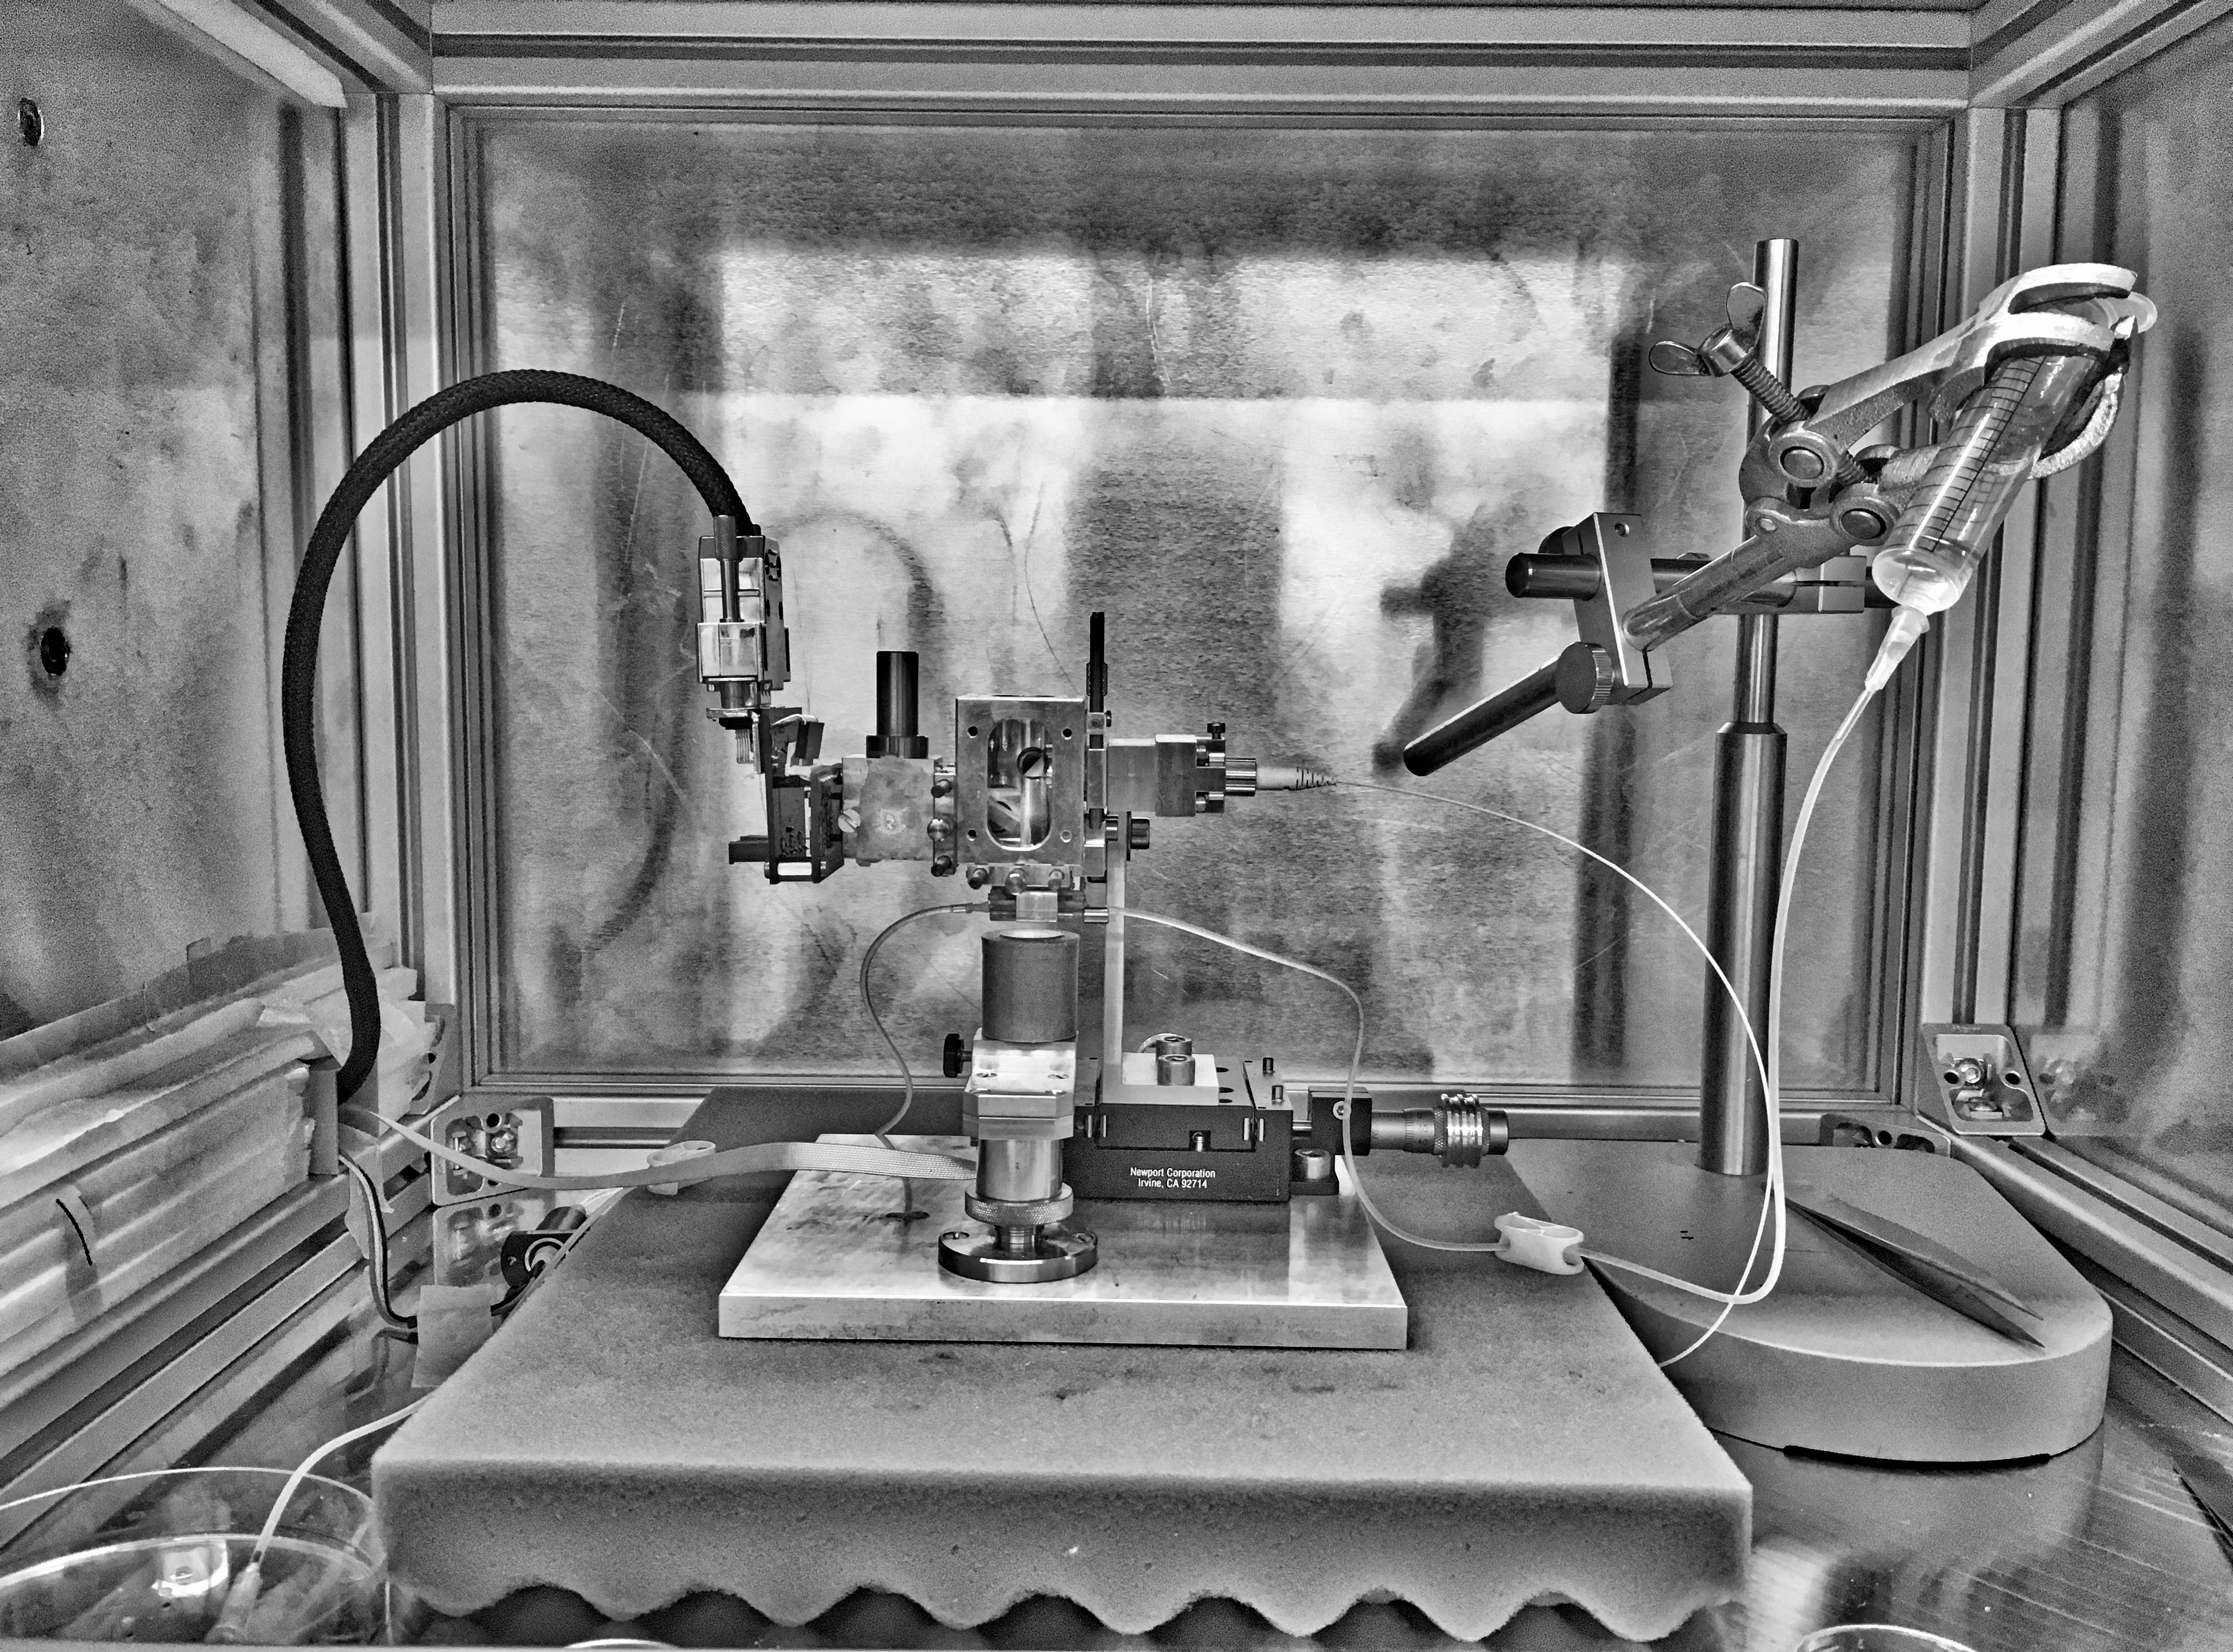
\includegraphics[width=1\linewidth]{Protot_firts.jpeg}%[height=40mm]
\caption{AFM Prototype 2016}
\end{figure}%

%\vspace{0.5cm}
\paragraph[center]{\center MASTER THESIS\\
 Master of medicine (M Med) der medizinische Fakultät Zürich\\
EPFL Lausanne, Faculty of Physics - Department of Physics of the living matter (LPMV)\\
Thesis Direktor: Sandor Kasas\\ Contact: massimiliano.bertacchi@uzh.ch\\ }%Matricl n°: 414 12 212\\


%/////////////////////////////////////////////////////////////////////////////////////////////

%\newpage
%\vspace{4cm}
%\begin{tabular}{m{6cm} m{5cm} m{3cm}}
                 %\hline
                 % after \\: \hline or \cline{col1-col2} \cline{col3-col4} ...
               %  \bfseries{Report Type:} & Intermediate & \\\\\\
               % \bfseries{Master Student:} & Massimiliano Bertacchi & \dotfill{} \\\\\\
                % \bfseries{Matricl n°:} & 414 12 212 ... & \dotfill{} \\\\\\
% * <massimiliano.bertacchi@uzh.ch> 2016-07-09T12:19:17.983Z:
%
% Mettere il vero numero di matricola (e guardare come si scrive in inglese)
%
% ^.
           %      \bfseries{Thesis Director:} & Dr. S. Kasas & \dotfill{} \\\\\\
             %    \bfseries{Date:} & \today & \\\\\\
 %               \hline
           %    \end{tabular}%
%/////////////////////////////////////////////////////////////////////////////////////////////

%\newpage
%\pagestyle{fancy}
%\fancyhead{} % Clear all header fields
%\setlength{\headheight}{24pt}

%\fancyhead[CE,CO]{{Master Thesis (2016)}} %

%\setlength{\headheight}{74pt}
%\setlength{\parskip}{0pt}
%\begin{quotation}%eventualmente: \begin{tabular}{m{8cm} m{5cm} m{4cm}}
		
     %   \setlength{\leftskip}{250pt} Ciò che rende bello il deserto é che, da qualche parte, nasconde un pozzo... \\
     %    \bfseries{} A. St. Exupery
%\end{quotation}
%%%%%%%%%%%%%%%%%%%%%%%%%%%%%%%%%%%%%%%%%%%%%%%%%%%%%%%%%%%%%%%%%%%%%%%%%%%%%%%%%%%%%

% * <massimiliano.bertacchi@uzh.ch> 2016-07-09T12:19:47.929Z:
%
% >  A. St. Exupery
%
% Spostare a destra e cambiare la citazione
%
% ^.
 %\end{tabular}%
\fancyfoot{} % Clear all footer fields
\fancyfoot[RE,LO]{\thepage}

\newpage
\tableofcontents %qui dovrei mettere l'indice

\newpage
\setcounter{page}{1}
\pagestyle{fancy}
\fancyhead{} % Clear all header fields
\setlength{\headheight}{24pt}
%\fancyhead[LE,RO]{\thepage} %
\fancyhead[CE,CO]{{Master Thesis (2016)}} %
%\fancyfoot{} % Clear all footer fields
%\fancyfoot[RE,LO]{\thepage}
%\fancyfoot[RE,LO]{\textit{\copyright M.Bertacchi}} %
%\fancyfoot[LE,RO]{\textit{%\today}} %

%%%%%%%%%%%%%%%%%%%%%%%%%%%%%%%%%%%%%%%%%%%%%%%%%%%%%%%%%%%%%%%%%%%%%%%%%%%%%%
\section{Introduction}
%%%%%%%%%%%%%%%%%%%%%%%%%%%%%%%%%%%%%%%%%%%%%%%%%%%%%%%%%%%%%%%%%%%%%%%%%%%%%%

In 1928 Alexander Fleming discovers Penicillin, the first antibiotic. This was probably the medical discovery with the most important influence for the improvement of men life expectancy.
In the following centuries scientists believed that the most important enemy of humanity was at his end battle. 
But bacteria unattended developed resistances against antibiotics ant the confrontation started again. 
\\
On 21 September 2016 UN approves a declaration\footnote{"At UN, global leaders commit to act on antimicrobial resistance" article of 21.9.2016} about the dangerous and unattended situation we are observing in our time with an important increasing of the resistance of bacteria to ATB. To underlain the importance of the problem Ban Ki-Moon said: 
"\textit{More than 200,000 newborn children are estimated to die each year from infections that do not respond to available antibiotics. An epidemic of multidrug-resistant typhoid is now sweeping across parts of Africa, being spread through water. Resistance to HIV/AIDS drugs is on the rise. Extensively drug-resistant tuberculosis has been identified in 105 countries (...). If we fail to address this problem quickly and comprehensively, antimicrobial resistance will make providing high quality universal health coverage more difficult, if not impossible}"\cite{Ban16}
%\footnote{ban Ki-Moon at the UN commit of 21.9.16 NY City}.
\\
Antibiotics resistance today is one of the most important medical challenges. Until today the clinical method to detect sensibility and resistances consist in making cultures and the time to have results is dependent on the rapidity of the reproduction of the investigated bacteria. This caused problems with slow growth bacteria because the results of the antibioramm could be read only weeks or month after the infection and as a consequence we have to treat the patients with empiric large spectrum antibiotics with the consequent risk of giving an inefficient antibiotic to the patient (with attended and unattended secondary effects) and to increase the general resistance of bacteria\footnote{cercare articolo sulla spiegazione dello sviluppo della resistenza
http://www.who.int/antimicrobial-resistance/events/UNGA-meeting-amr-sept2016/en/}.
%citare l'aticolo e aide memorire dell'UNO che ho salvato sulla penna

For this reason is really important to adapt the utilization of antimicrobial medicament and especially prescribe them only to patients that could really take advantage. How described in the intention of UN is capital to limit the distribution and random utilization of this type of medicament as really often it is used like a first respond medicament to treat suspected or minor infection. 
But the great limitation for an optimal utilization %(o sinonimo) 
of antimicrobial is the identification of their efficacy in useful time. Sometime it is not so easy, or impossible to have an antibiogramm before the first treatment. More complicated is the situation with slow  growing bacteria that that need more weeks or months to have a positive culture and the determination of the MIC\footnote{Minimum Inhibitory Concentration}, in this case an empiric treatment is necessary (obbligato).
\\
The work of S.Kasas Group is focused on developing an AFM prototype able to detect activity of bacteria metabolism and their movement to evaluate the efficiency of antibiotics. This prototype\footnote{see article 1 lpmv epfl} works as a really sensitive movement sensor and is able to detect the movement or metabolic activity of a sample of bacteria attached on a cantilever\footnote{microscopic golden tip see images}.
If the antibiotics is efficient we see the diminution or the disappearance of the signal of the metabolic-induced vibrations. In this way we have results in some minutes instead of days, weeks or months. 
\\
The utilization of an AFM in this way could be a great revolution, because of his rapidity of the results it could avoid the utilization of inefficient ATB with non-sensitive microbes and also permit to calculate the MIC really slow growing bacteria in some minutes or hours.  
\\
There are also other applications that could be imagined for this AFM-prototype: for example in the same way as we use it for bacteria and ATB we could use it to detect the efficacy of chemotherapy on tumor cells\footnote{cercare articolo?}\cite{articolosconosiuto1}. An other application could be the characterization of the microbe metabolic specific signal that could permit us to diagnostic the microbe family that cause the infection (mind network). 
One more spectucular aplication of the AFM in this way is the detection of living microbes in hostile environments or for even detect live in others planets\footnote{citare articolo o proposal del progetto con la nasa}.\cite{articolosconosciuto1}. 
%magari citare anche Burkh. il suo discorso all'UN

%%%%%%%%%%%%%%%%%%%%%%%%%%%%%%%%%%%%%%%%%%%%%%%%%%%%%%%%%%%%%%%%%%%%%%%%%%%%%%
\section{Work Objectives}
%%%%%%%%%%%%%%%%%%%%%%%%%%%%%%%%%%%%%%%%%%%%%%%%%%%%%%%%%%%%%%%%%%%%%%%%%%%%%%

The first goal of my work is the improvement of the AFM and protocols to permit a clinical utilization of the AFM as a diagnostic tool for the antibiotics resistance detection. 

To get this clinical application I have identified two critical points: the first one is to define a reliable procedure to detect the metabolism activity of the microbes and in this way the efficacy of the antibiotics for different type of microbes (different type of bacteria, yeast and odes cells). The second critical point is the necessity of a calibration of the prototype that permit us to have a comparable output signal all along the experiment (specially for long experiments) and that hallow us to compare more experiments made in different conditions. 
\\
To answer the first point I used the prototype with different type of bacteria (in particularity slow growing one like Bordetella Pertussis) and yeast to detect their sensibility or resistance to the ATB.
I have to underline that the goal is not the characterization of the bacteria resistance\footnote{see work of Ines Vilalba} but to the improve the utilization of the prototype focused on a clinical utilization. 
\\
At the same time I tried to point out the limitations of the AFM and I tried to solve them in order to have more specifics and reliable results.

I developed this second point in two ways, the firs one is a theoretical model to normalize the signal collected in different situations. 
One of the most important problems in AFM experiments in general is that the esperiments are not quantitatively(non so se si puo dire) comparable. The conditions (like position of the cantilever, temperature, refraction and density of the fluid, position of the laser and so on) are continually changing between different experiments and along the same experiment its self. For this reason I tried to use the FFT (Fast Fourier transform) to have a calibration of the "sensibility" of the prototype and I tried to write a logarithm for the normalization of the output signal.


\subsection{Biological Experimentation}%-------------------------------------
The biological part is focused on the utilization of bacteria as B. Pertussis (different strain), E. Coli, S. Aureus and one type of yeast (Saccharomyces) to validate the utilization of the AFM-prototype for detecting the resistance and susceptibility of bacteria on ATB. For this reason I made about 15 experiments\footnote{Each experiment is coded using the date of the day in witch the experiment has been made} to evidence the capacity of the prototype of detecting the susceptibility of the microbe to ATB and to identify all the problems that need to be corrected before a clinical application. 
I try to do the experiments with the same accuracy we may imagine in a clinical utilization and to use processes that could be possible also in a hospital and not only in a experimental lab. 
I made the experiments in toto: culture of the bacteria, cleaning, isolation and fixation of the sample on the cantilever, alignment of the laser, collection of the data and data analysis. 


\subsection{Algorithm for the normalization of the Signal} %----------------------------
The calibration of the prototype and the normalization of the signal is one of the most complex problem with the utilization of an AFM when we use it in a different way as imaging. For example in our case, the utilization of the cantilever as a movement sensor has grates output variations between different experiments.
The classical approach is the use of some parameters, like the laser deflection, to estimate the conditions of the AFM. (.......Trovare un articolo che parli della calibrazione) but are inefficient and not enouth precise to make a correction of the signal. 
As the AFM is used as a movement detector (which give us a quantitative information) and not as an image microscope (that give us a qualitative information) we need to have a measure of the intensity of the Signal. To do that I thought to use the FFT at a time (t) to have a reflection of the sensibility-state of the AFM. This idea is supported by the observation that the good alignment and conditions of the prototype (that have as a consequence a high sensibility of the movement) are reflected in a well-defined resonance pic in the FFT \footnote{mettere un immagine di un FFT standard}. 

\begin{figure}[h]
\centering
		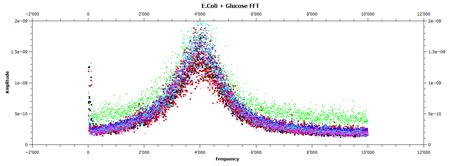
\includegraphics[width=1\linewidth]{FFT/FFT_dacambiare.jpg}%[height=40mm]
\caption{FFT esempio per vedere il picco da cambiare} %attento cambia questa immagine 
\end{figure}%

This motivated my to better study the FFT and his correlation with the sensibility of the prototype. 
Starting from some data collected from M.I. Vilalba\footnote{citare il lavoro di Ines}, end some experiments I made, I tried to use the FFT as a continuous indicator of the sensibility of the AFM. The goal was to find a correlation between the FFT and the signal and in a second time use this correlation to correct the amplitude of the output signal to a theatrical optimal set point of the AFM. %magari spiegare meglio 
In this way we could archive (!!) two goals: the first one is to know "how good" is our signal and then correct it to a "theoretical optimal Signal" (with an indication of the error range), the second one is that we could have a comparison between the different experiments.  %completareeeee

\subsection{Minor Objectives}%-------------------------------------------
Qui bisognerebbe mettere sia gli obbiettivi secondari come l'identificazione di rumori strani nel segnale e l'isolazione meccanica
Un esperimento che si può citare é quello della punta colorata per la detezione del rumore elettronico

The second aspect is the fiscal isolation of the prototype with the limitation of fiscal and electronic noise that are one of the most important source of difficulties in the analysis of the signal.
%%%%%%%%%%%%%%%%%%%%%%%%%%%%%%%%%%%%%%%%%%%%%%%%%%%%%%%%%%%%%%%%%%%%%%%%%%%%%%
\section{Methods}
%%%%%%%%%%%%%%%%%%%%%%%%%%%%%%%%%%%%%%%%%%%%%%%%%%%%%%%%%%%%%%%%%%%%%%%%%%%%%%

\subsection{NanoAFM Technology}%------------------------------ SVILUPPARE MEGLIO E CITARE CHI FA QUESTE COSE
The technology we used for this work has been described by Kasas and all.\footnote{1o articolo su AFM}. We used a simplify AFM prototype optimized for the isolation of the movement of bacteria that are fixed on the cantilever. 
As well as commercial AFM a combination of mirrors deviate a laser pointer on the cantilever. The reflection of the laser on a photodiod permit to identify the position of the cantilever (angle of inclination) an in this way his movement (see image schema fatto da me).
%\includegraphics[width=0.25\textwidth]{UN} INSERIRE SCHEMA DI COME FUNZION L'AFM
\\After the introduction of the cantilever in the chamber and before starting the experiment we have to align the laser and set his intensity\footnote{usually set at 49.00mA} at the same time we have to set the position of the cantilever, to make this two processes we have a camera under the chamber that permit us to see the position of the cantilever and that one of the laser. In this way we can align the two in a optimal position\footnote{W.Chomiky is working at the automation of the alignment process so that in clinics this step it would not be necessary}. An optimal alignment is reached when the laser is good centered on the distal point of the cantilever so that the vibrations are more perceived. Also important is that the final spot of the laser is centered in the middle of the photodiod (we can modify that with the inclination of the mirror and the position of the photodiod). 
The laser must be in the center of the photodiod to have the maximal sensibility of the movement in every direction and avoid the saturation by reaching the borders. To align that we use a prism that make an optical reflation of the laser on a screen that represent the "position of the laser on the photodiod\footnote{we tried monitoring this position with an optical camera to detect the movement without the photodiod}. The second way to set the initial position of the laser is to move the spot to the two opposite limits of the photodiod. We will find two curves on the two components of the output signal (L-R component and Botto-Top component). The spot in in the optimal position when the starting value is set in the middle of this two extremities (cambiamento di pendenza).
These two ways of alignment could be automated: with the optical monitoring of the spot we could have a continuous correction of the mirrors to have the spot in the optimal position (but it would introduce an important variability in the experiments) the second could be more adapt to our type of experiements with an automatic calibration of the position of the spot after having put the cantilever on the chamber. The softer could automatically move the spot on the limits and detect the central point. 

\begin{figure}[h] 
\centering
		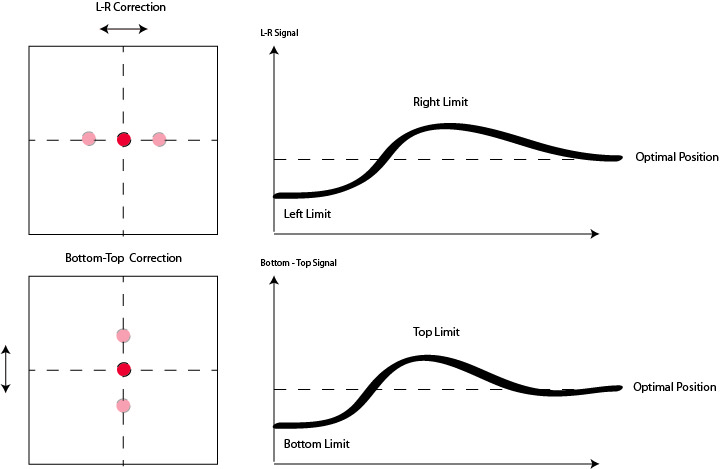
\includegraphics[width=0.6\linewidth]{FFT/Spot_position2.jpg} 
\caption{Calibration of the spot position on photodiod} 
\end{figure}%     

The chamber has two small input and output tubes that permit to fill the chamber and to change the liquid during the experiment\footnote{in the past we tried to make experiments with a small continuous flow in the chamber but in this case we prefer to make the experiments with a stable liquid without flow in order to limit the noise}. \\
We take a picture of the cantilever before and after each experiment and we recorded also the start-FFT and the end-FFT (in some special case we recorded more intermediate FFT to monitor the sensibility and the state of the prototype).
%%%%%%%%%%%%%%%%%%%%%%%%%%%%%%%%%%%%%%%%%%%%%%%%%%%%%%%%%%%%%%%%%%%%%%%%%%%
More description of the function of the AFM (...).
\\
\\
The reasons of the development of a prototype instead of using a commercial AFM\footnote{Parallel experiments on commercial AFM are actually made by P. Stupar at LPMV EPFL} are:
\begin{itemize}
\item The prototype production has an important reduced costs compared to a commercial AFM: 5k vs 200k
\item We optimize the function for movement detection instead of imaging 
\item We simplify the utilization and automatism for a simple clinical application 
\item We have a simple, sterile and isolate environment that permit the utilization of dangerous bacteria and avoid contamination of different samples.
\end{itemize}

\subsubsection{Isolation}
It is really important to isolate the prototype from external movement, vibrations and electric noise. For this reason we adopt some strategies to isolate and ameliorate the sensibility of the prototype in order to better detect the cantilever movement. 
The first and more important action (??) is the physical isolation of the prototype. In some case the prototype could be placed on a stabilized table\footnote{special table able to reduce the vibration and isolate the objects from the environment}. We decided to use the prototype on a normal table and to isolate it in a different way as this type of table is normally not available in an hospital or a medical practice. We set the prototype in a metal box surrounded with isolation material on the walls. I made some experiments to validate the quality of this isolation. This series of experiments are not discussed in this work\footnote{The results are in the attachments}. 
\\
The second way to isolate the signal is to use an electronic filer on the signal and select the windows of frequencies that correspond better to the cantilever movement and cut off the electrical noise of the electronic equipment.\footnote{In all my experiment no frequency filter is applied}.

%descrizione degli esperimenti sull'isolazione

\subsubsection{Equipement}%------------------------------
%The most important equipment I used for all the experiments are listed here: %guardare meglio come scriverlo e se scriverlo
\begin{itemize}
	\item Usual laboratory (P2)\footnote{security level BSL-2} equipment
    \item AFM Prototype 
    \item Optic mycroscope with ximea camera (verifica la camera)
    \item Apparecchio calcolo concentrazione 
    \item Plasma cleaner: I used a PlasmaCleaner to clean old cantilevers used in experiments wihout bacteria attached on it. We consider that the use of Plasmacleaner with biological material is not jet optimal to use cantilevers for more times, we prefer to use Piranha solution \footnote{Dannis, piranha solution sulfuric acid (H2SO4) and hydrogen peroxide(H2O2)}
    \item Altro...
      \end{itemize}
      
\subsection{Data Analysis}%-------------------------------------
The output signal of the Prototype is the value of the position of the laser on the Photodiod transformed in intensity. This value on the time is usually transformed in a variance pro Chunk. So we calculate the variance of the signal in a variable period of time.
%inserire un immagine con ad esempio un segnal eper 1chun/1sec
A second parameter that is sorted out of the signal is an FFT\footnote{Fast Fourier Transform} that can tell us which frequencies are presents in our signal and in with amplitude\cite{ articolo sugli FFT}.
This FFT is useful to understand the sensitivity of the cantilever in each moment. It is like a instant-photo of the conditions of the prototype in a defined moment. If the resonance pic of the cantilever\footnote{ca. 3-4kHz} is present it permit us to understand that the movement of the cantilever are good detected by the prototype.If there are some interference (most of them are electronic noise) we will have some important spikes in other frequencies. The FFT analysis will be discuss later. The signal it self is normally analyzed as a variance of the signal and we consider his amplitude and then his variation along the time.
(...)%inserisci l'immagine di un FFT
\\Each FFT will be analyzed in Matlab with a function\footnote{the function has been written by me starting from the Matlab tool of Gaussian-fitting} that fit the curve of the FFT (cutting his extremities to eliminate the noise) and automaticale isolate some parameter that I used like index of the state of the prototype. 
\\Exemple of parameters sorted out of the function: 
\begin{itemize}
\item Maximum point
\item Rsquare\footnote{The Rsquear is a good parameter to know if the the FFT is good adapted to the Gauss curve}: This i s a good indicator of how good is the FFT and if there is a good resonance Pic. It is a better parameter than the  
\end{itemize}
One of the most difficult point of the analysis was the treatment of big Data. The Signal file are in a range from 100Mb to 1GB pro file and to treat them it is necessary to split the files in many smaller parts ore transform the Signal in a Variance and use this one (the size is considerably reduced). 

\subsubsection{Software}%------------------------------
To analyze the collected data we use a program written in LabView\footnote{tha analysis-program is an implementation of a program written by Givanni Longo} that permit us to see the variance of the signal pro defined chunks and to apply some filters of the frequency\footnote{not frequently used}. An other important tool for analysis was Matlab that we use to analyze the signal, to have the variance vector and the most important thing was used for the analysis of FFT that permit to evaluate the signal quality and to make the corrections that I describe in the chapter about the calibration theory\footnote{verificare che si chiami in questo modo quando finisco di scrivere e guardare se sono stati utilizzarti altri programmi}.Finally the Thesis has been written with LateX\cite{documento guida Latex}.

\subsection{Preparation of Bacteria and Antibiotics}%------------------------------
\subsubsection{Bacteria} %completare con protocollo
I will describe the basic procedure to prepare bacteria and ATB that are common used in our experiments. Many variations has been made in some special experiments, those exceptions will be described separately in each specific experiment. \\ Bacteria are normally cultivate (from a frozen starting sample) for one or two days (to have a good concentration and to be sure to have a pure strain (this passage has to be replaced in clinics by the isolation of the infect plasma or other collected liquid of the patient). The cultivate bacteria are washed from the culture medium\footnote{Specific for each bacteria, described later} with four subsequent centrifugation (80rp for 5min) and wash with PBS \footnote{Phosphate Buffer Saline solution}. At the last wash we calculate the concentration of the bacteria (we normally use a concentration of 300...\footnote{calculate with...maschine} ).
\\We add some drops of glutaraldehyde on the cantilever for 15min to make it more adhesive. After it we have two possibilities to let it dry in ambient air or to wash it with pure water (we use some drops of pure water indirectly on the cantilever). We normally prefer to clean it with pure water and let it dry for some seconds. 
Than we add some drops of concentrate bacteria on the cantilever for 30min.
At the end of this time we put the cantilever in the prototype support in a free chamber. After the chamber is closed we fill the chamber with a basic solution dependent of the type of the experiment (normally we use the specific culture medium of the bacteria).
\\After the alignment of the laser we prefer wait 5min before beginning to  record the movement, so we let the time at the cantilever to stabilize its self and stop the vibrations caused by the entry of the fluid in the chamber. We normally wait always 3min in each change of liquid in the chamber (even if the flow is really small) to avoid turbulence in the fluid that could cause some movement of the cantilever.

\subsubsection{Antibiotics} %scrivere una breve introduzione al protocollo + protocollo
Filtration\\
(...) With Bordetella we used: 
\begin{itemize}
\item Erytromycin 
\item Clarytromycin 
\item Mix ATB: Trimethroprim and Sulfamethaxole (1:19)
\item Peniuillin
\end{itemize}

\subsection{Experiments}%------------------------------
\subsubsection{Comparative activity of ATB, water, alcohol and medium}
At first we need to verify that the activity of ATB, medium or others liquids in the chamber do not cause significant impact on the cantilever movement\footnote{for it was also a first opportunity to use the prototype and understand how to set it optimally}.
To do that we made some comparative experiments to compare their activity. We use the cantilever free\footnote{no bacteria or molecules attached on the cantilever} in the chamber and we recorded his movement in different medium. 
\\The first experiment\footnote{06.07.16} was simply to compare t6he activity of water (control) with a solution with ATB\footnote{quale ATB?} with MBC\footnote{Minimum bactericidal concentration, that is more important that the MIC, importante da sottolineare che l'MIC non é la concentrazione letale} concentration diluted in Water. Each solution is recorder for 10min. In the same way a compare\footnote{06.07.16} the activity of Medium (SS)\footnote{in this case I use SS that is the medium for Bordetella Pertussis}in two different concentration (50\% and 100\%) and one ATB (Erytromycin). In a last experiment\footnote{07.06.16} I compare: Water, Medium and two different ATB\footnote{Eçrytromycin and a Mix ATB comnposed by T and S ...}

\subsubsection{E.coli}
The experiments with E.Coli could be used as a "gold standard" as it is a large bacteria with an important and rapid metabolism (rapidly growth Bacteria...) and for this reason his activity is easy to detect  and in addition the culture is easy and very rapid. 
I used E. Coli for two experiment\footnote{I used E. Coli in a student project in 2013 to evaluate the possibility of using an AFM with a continuous flow of medium in the chamber}\cite{ilMioLavoroReport2013}. The first experiment\footnote{11.07.16} was thought just to detect the stop of the activity of the bacteria. I use the standard procedure\footnote{described before p.4 General preparation of Bacteria} with E.Coli on the cantilever and I made 15min of recording. After this time I add in the chamber an high concentration of alcohol to kill the bacteria and observe the modification of the metabolism activity. 
The second experiment\footnote{14.07.19} with E.Coly was the idea to detect the increase of the metabolic activity with some nutrients (glucose) in the solution to better identify the metabolic caracteristics of E.Coly and the capacity of the prototype to detect the modification of the metabolism. (Procedure... e rifare l'esperimento in laboratorio...). 

\subsubsection{B. Pertussis}
The experiments\footnote{the experiments described below are made by my but they are the result of a continuous discussion with I. Vilalba and a comparison with his work} with Bordetella Pertussis are the main part of my work. Bordetella is a small slow growing bacteria and could present resistance to ATB. For this reason we chose to utilize this bacteria as a good simulation of a challenging clinical situation. %forse in intro 
\\The first experiment\footnote{28.07.16} is a simple observation of Bordetella attached on the cantilever after administration of the mix-ATB\footnote{Trimethroprime 80$\mu$g/ml and Sulfamethacole 1:19} at MIC concentration\footnote{MIC concentration for the Mix-ATB Concentration balanced on Trimethroprim = 80ug/ml that means:  S-300ul (at 20mg/ml) and T-16ul at (19.6mg/ml)}. At the beginning Bordetelle is sorraunded by the medium (SS\footnote{descrivere SS?}) for ca. 25min and at this point we add the ATB (at this time I have adjusted the position of the laser because the sensibility was not optimal\footnote{we can consider the t-0 the moment in which we start the ATB without consider the first part}). After the subministration of the Mix-ATB\footnote{Mix of Trimethroprim and Sulfamethaxole 1:19} I made ca. 3 hours of recording. At the time t-2h20min it could have been some interference caused be my manipulations on the table. \\


The same experiment  (always with the mix-ATB in MIC concentration) has been repeated\footnote{02.08.16} but with a more long time of monitoring (ca. 7 hours) to see if we can better evidence the effect of the ATB.

\begin{figure}[h] %[h]= here, [t] = top % capire come posizionare le immagini nella posizione giusta del testo. 
\centering
	\begin{subfigure}{0.245\linewidth}
		\centering
		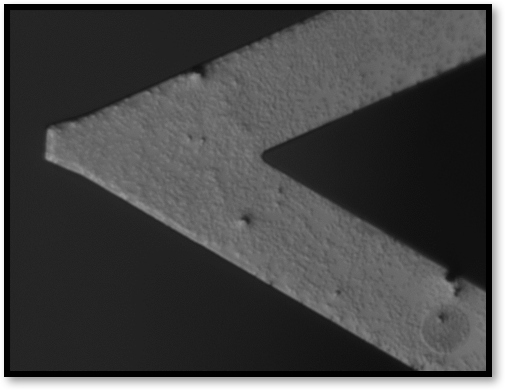
\includegraphics[width=1\linewidth]{Cantilever/BP_Canti_2807}%[height=40mm]
		\caption{}\label{fig:2807}
	\end{subfigure}
	\begin{subfigure}{0.245\linewidth}
		\centering
		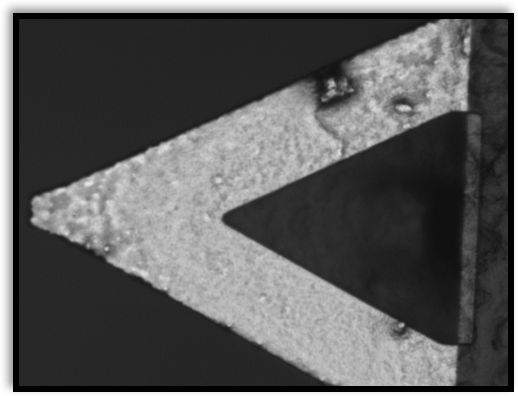
\includegraphics[width=1\linewidth]{Cantilever/BP_Canti_0208} %[height=40mm]
		\caption{}\label{fig:0208}
	\end{subfigure}
\caption{BP on cantilever before starting experiment \subref{fig:2807} BP 2807, \subref{fig:0208} BP 0208} 
%\SIlist{10;100}{\nm} ballistic and diffusive devices.
\end{figure}%
In the first 120min of the experiment BP\footnote{Bordetella Pertussis} is surrounded by the medium. It was not easy to have a good sensibility and for this reason I have recorded three times the FFT that could give us an idea of the sensibility of the prototype in the first steps. After that I had the ATB and we start the long recording for 5h. At the end of this long ran I wash the chamber and I felt it with ultra-pure-Water to have a zero signal comparison. At the end of the experiment I take a picture of the position of the Laser on the cantilever with an optical Camera on the Bottom of the prototype. I tried to correct the position and I observe the modification of the signal at the end of the experiment (always in Water) after this correction. 

\begin{figure}[h] 
\centering
	\begin{subfigure}{0.245\linewidth}
		\centering
		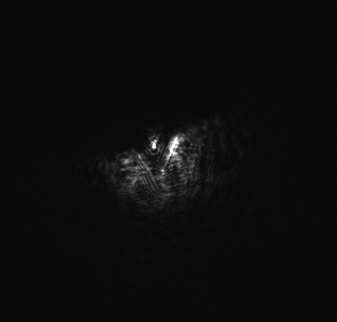
\includegraphics[width=1\linewidth]{FFT/Lp_0208_end}%[height=40mm]
		\caption{}\label{fig:2807}
	\end{subfigure}
	\begin{subfigure}{0.245\linewidth}
		\centering
		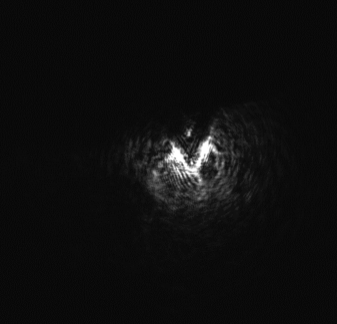
\includegraphics[width=1\linewidth]{FFT/Lp_0208_correct} %[height=40mm]
		\caption{}\label{fig:0208}
	\end{subfigure}
\caption{Laser position \subref{fig:2807} Lp begin, \subref{fig:0208} Lp end} 
%\SIlist{10;100}{\nm} ballistic and diffusive devices.
\end{figure}%
This was necessary to be sure that the decreasing of the Bacteria activity was associated with the effect of the ATB and not to a lost of sensibility of the prototype that could simulate an apparent decrease of the Bacteria movement. 
%...
\\
In the third experiment\footnote{16.08.16}, that is similar to the past two ones, we have three steps: in the first we let the cantilever with BP in medium\footnote{this medium is an SS modified, it consist in the normal SS with the addiction of a minimal concentration of alcohol that is the same concentration we add to the ATB to dissolve the ATB in the solution. This concentration (XXY) is really low and has no influence on the activity of the Bacteria} for ca.30min, than we add the MIC Mix-ATB for 1h. Than we change the liquid in the chamber by introducing the same Mix-ATB always at MIC to compare if the detected activity has variations due to the manipulations and not only by the activity of the ATB. After a second hour we repeat the same procedure by injecting for a third and a fourth time the ATB at MIC. The last step of the experiment was to change for a last time the liquid by injecting the ATB at a MBC\footnote{Minimal Bactericidal Concentration} in order to see if a greater concentration of the ATB is able to decrease more the refractory activity. 
\\
I made an other experiment\footnote{17.08.16} to compare the activity of BP in medium, ATB MBC and Water (...) experiment to be repeated.\\
I performed a last experiment\footnote{Experiment code: 170816} with a resistant strain of BP\footnote{mettere il nome della forma resistente utilizzata}. For this experiment I used two ATB, the first one () has no effect on the rBP as it is resistant and the second one (the mix-ATB) the is theatrically efficient also against this strain.
We began with the BP in medium (SS) for XYmin, then we add the inefficient ATB (name) and we recorded for xymin. Finally we use the mix ATB (concentrations?) that should be efficient and we recorded the signal for xy min. 
%specificare il lavoro di Ines per determinare l'attività degli ATB prima di utilizzarli. Cosi come lo studio delle concentraizoni...

\subsubsection{Saccharomyces}
In this experiment\footnote{Experiment Code: 12-130716} we use Saccharomyces\footnote{One specie of yeasts that is a sugar fungus} that has an important diameter compared with bacteria (Saccharomyces 2-8\textmu m vs 1\textmu m of BP) and a more active metabolism. 

\begin{figure}[h] 
\centering
	\begin{subfigure}{0.3\linewidth}
		\centering
		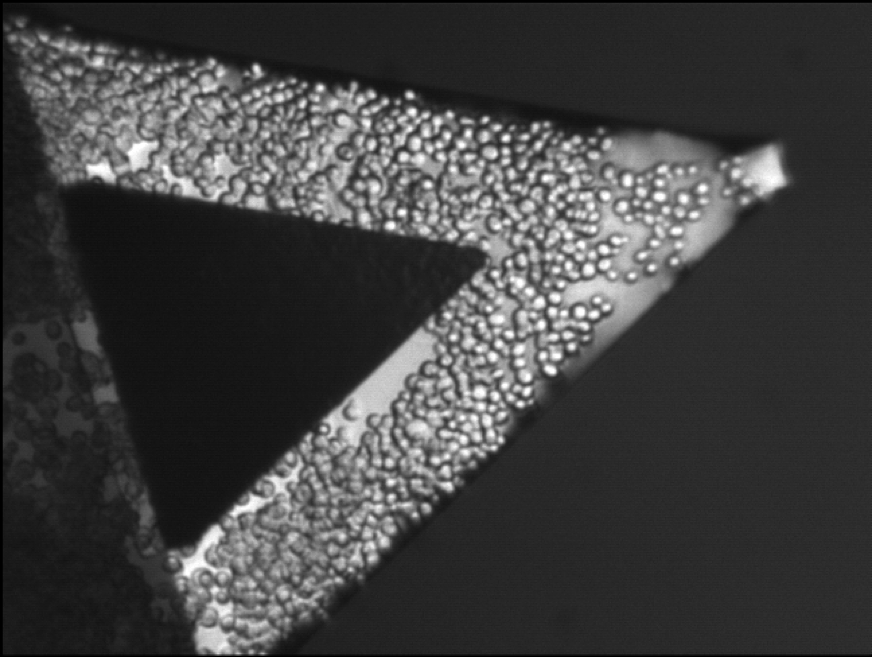
\includegraphics[width=1\linewidth]{Cantilever/Saccharomyces1}%[height=40mm]
		\caption{}\label{fig:SC_cantilever_B}
	\end{subfigure}
	\begin{subfigure}{0.3\linewidth}
		\centering
		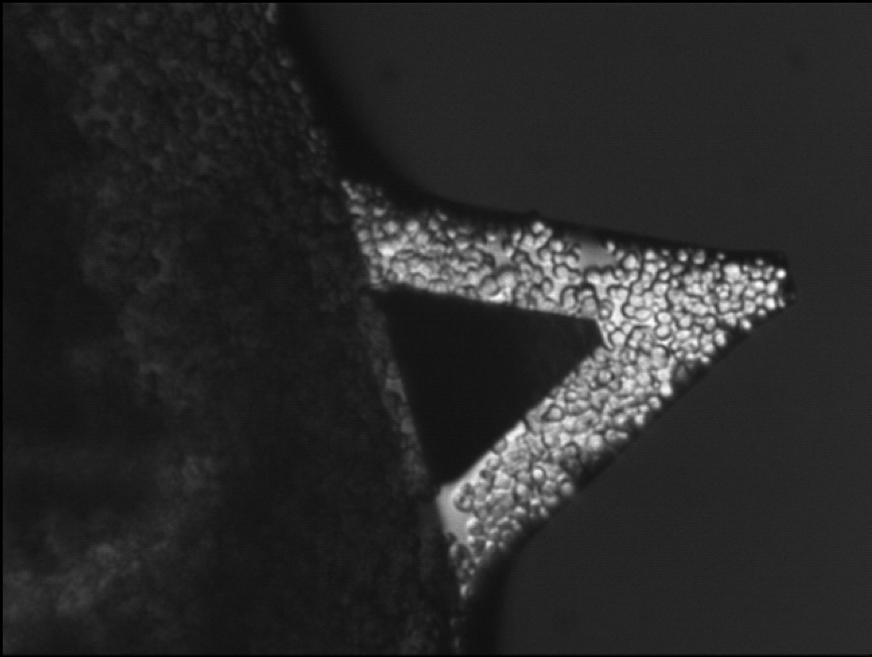
\includegraphics[width=1\linewidth]{Cantilever/Saccharomyces2} %[height=40mm]
		\caption{}\label{SC_cantilever_A}
	\end{subfigure}
 \caption{Saccharomyces on Cantilever \subref{SC_cantilever_B} Cantilever B (used for experiment), \subref{SC_cantilever_A} Cantilever A} 
  \end{figure}

The preparation of Saccaromyces is (...)
We can imagine this experiment in three steps: 1. Starting  phase 2. Long time following 3. Ending phase
In the starting phase we fixed Saccaromices on the cantilever and we let it for 5min surrounded by PBS\footnote{definizione di PBS} and we recorded the references activity. Then we put some YPD\footnote{specfic medium for Saccaroyces} in the chamber to increase the SCM activity. After a recording of ca. 1h I started a long time recording during of ca. 7h without any manipulations.  At the end of this phase we observe some bauble of air and some agglomeration of yeast. After having changed the medium of the chamber (without open it) we enter the Endig phase where we add some alcohol at 50\% to see if we could decrease the activity of the yeast metabolism. After ca. 20min we ad 100\% Alcohol in the chamber for 13min and change the medium with other 100\% alcohol and observe the activity for others 20min. 


\subsubsection{Free cantilever and bacteria in suspension} %MOLTO IMPORTANTRE per l'aspetto clinico

In the following experiments we do not attached bacteria on the cantilever, instead we let the free-cantilever\footnote{without bacteria attached} in the chamber, surrounded by the specific medium of the bacteria. After a short moment of recording in witch we let the time to stabilize the cantilever and to have a zero-activity reference, the bacteria are introduced in the chamber in a suspension (with a controlled density of bacteria) and the activity is recorded in this conditions. \\
Preparation of the bacteria suspension: \\
The bacteria are (…) %completare le preparazioni
We put the same bacteria (frome the same culture ore clinical isolation) in two tubes: the first one is mixed with the specific medium and the tube is defined as the \textit{alive bacteria} (microbe), in the second tube we put the bacteria in a solution with a test-substance (like ATB, Alcohol, …) and we attend that the substance act on the bacteria. After a defined time (in our experiment are 15min * verificare il tempo) we centrifuged and wash the bacteria from the solution and we suspended the bacteria in the medium again (the centrigugation and wash process is repeated 4times VERIFICARE). At this point is important to have the same concentration of alive and dead bacteria in the two tubes to not false the activity. We normally used a concentration of 300yx/yx. But we manage to do some experiments with different concentrations in the future to observe the changes. 
\\
The first experiment\footnote{Experiment code: 080816} will compare a alive-sample of BP with a dead-sample of BP killed with alcohol\footnote{Hands-alcohol}. We used the hospital hands disinfectant (75\% alcohol) to kill BP by letting the bacteria supended in the solution for 45min (verificare). The alcohol component is washed away by the subsequent centrifugal and suspension of the bacteria in medium. Anyway some molecules could remain in the final solution even if strong diluted.\\
We recorded for 40min the free-cantilever in medium as a zero-activity reference (also to be sure that the medium was not been contaminated). Than we ad the alive-bacteria suspension in the chamber and we recorded the activity for 15min. At the end of this time we changed the medium with a really slow flow without voiding the chamber\footnote{there are more opportunities to change the medium. Ines Vilalba preferred voiding the chamber and cleaning it with some important flow to be sure that the chamber was not contaminated by the alive bacteria. I prefer to simulate a clinical application with a less complicated system and avoiding an important chang of conditions that could modify the sensibility of the prototype.} for 3min to have a complete change of the medium in the chamber, Afeter 2 min by the administration we have a stable cantilever and a new zero-activity that we recorded for others 15min to be sure that in the chamber there is not residual activity of the alive-bacteria. The last step is to introduce in the chamber (always with a low flow for 3min) the dead-bacteria solution and we recorded the activity for 15min. \\
As the hands-alcohol seems to make some interference to the signal\footnote{probably containing some molecules that interference with the cantilever} we made a second experiment\footnote{Experiment code: 110816} with the same procedure but we use pure 75\% alcohol to kill bacteria (instead of the hospital hands-alcohol disinfectant).\\
Also the pure-alcohol seems to have interactions with the cantilever (as we observed an increasing of the activity of the “dead-bacteira”) and we needed to try a third experiment\footnote{Experiment code: 120816}  in witch we killed bacteria with an ATB instead of using alcohol. The dead bacteria preparation has been obtained by letting bacteria 1h (verificare il tempo) in the mix-ATB suspension and then washed and suspended again in medium. The classical schema is applied: 15min medium-alone, 15 medium alive-bacteria, 15min medium, 15min dead bacteria. \\
In the last experiment\footnote{Experiment code:120816} with BP we prepared two “dead-bacteria samples”. The first one using the Mix-ATB and the second one using Clarytromycin (we use a strain of BP sensible to the two ATB), we use the same procedure described before so there we do not have any ATB in the chamber as the bacteria are re-suspended in medium. As in the past experiments we measured 15min of medium, 15min alive-bacteria, 15min medium, 15min dead-bacteria with Mix-ATB, 10min medium and 15min dead-bacteria with clarytromicin. 
\\I repeated the experiment with some others Bacteria like Stafilococcus Aureus (SA) and E.Coli. For this bacteria we used the same procedure described for BP (we used LB instead of SS as a medium). With SA I made two experiments: the first\footnote{Experiment code: 080816} using Hands-alcohol like with BP. 

So I prepared the dead-bacteria sample with hand alcohol (suspension for 1h (VERIFICARE)) and then I centrifuged and wash the bacteria for (x times) to not have alcohol in the chamber. The recording schema is: 10min medium (LB), 10min alive bacteria, 10 min medium, 15min dead-bacteria. As we found the same problem as with BP and hands alcohol we repeated the experiment with pure alcohol. 
This time\footnote{Experiment code: ST090816} the recording schema is:  5min medium (LB), 15min SA-alive, 15min medium, (15min dead bacteria, sample with problem, 15 min medium), 15min dead bacteria. 
 
Finally we repeated the experiment with pure alcohol (75\%) with E.Coli\footnote{Experiment code: 090816} following the recording schema: 10min medium, 10min \textit{alive-bacteria}, 10min medium, 10min \textit{dead-bacteria}
(FORSE SI POTREBBE COMINCIARE CON E.Coli E SA E POI FINIRE CON BP).


\subsection{Algorithm for the normalization of the Signal}%-----------------
At first it could be interesting to describe the studies we made on the FFT\footnote{magari citare arcolo FFT}. In the following graphs %(mettere i disegni schemi di Ines)
we can see that the position of the laser on the cantilever modify the shape of the FFT. %dettagliare meglio guardando il lavoro di Ines
But we still do not know the correlation with the signal (the goal is to find a mathematical approximation that could describe this correlation) and we still do not have a good description of the FFT in the differents situations (position of the Laser, temperature, viscosity of the medium, different type of cantilever, ...).
In this work I will focus on the first point so the correlation between the FFT and the signal but it will be interesting to study more deeply the TFF modification in different conditions. %forse questo pezzo va anche nell'introduzione
\\I decided to use a standard physical input signal (a small mechanical vibration on the base of the prototype) as a standard measure of the signal and use it to observe how the output signal (that represent the vibration detection of the prototype) change in different conditions\footnote{I concentrate my self on the laser position and I do not consider the other parameters in this work} that change the sensibility (described by the FFT shape) of the prototype.
\\%mettere immagine iniziale con le differenti vibrazioni
I recorded the FFT of each vibration (that are every time the same, but are perceived every time in a different way). If we detect a good parameter to quantify the quality of the FFT ("how much the prototype are sensible") we could set this value in a graph in correlation with the signal intensity (the vibration detected amplitude). The study of the FFT and the code I write to study them are in attachment and is not described here. I isolated three parameters that could be used to quantify the sensibility of the prototype: 

\begin{itemize}
\item The maximal point of the pic
\item The high of the pic (distance between the base of the FFT ant the maximal point)
\item Rsquare of the Gaussian fitting of the FFT\footnote{also this code is described in attachment}
\end{itemize}

% il prossimo passagio rest acomplicato, bisognerebbe spiegarlo meglio
At this point I recorded 7 Vibrations in different conditions and the correspondent FFT. I isolated the median amplitude point of each vibration (V1,V2,V3,V4,V5,V6,V7) and for each vibration I made a FFT analysis.%insierire le immagini degli FFT. Verificare il nome che do alla variabile FFT e quella dell'ampiezza
The FFT analysis (that I normally made in routine for each experiment) are a fitting of the FFT and the isolation of some parameters like: Max-point, r-square and the Gaussian-high.
I drow a graph with the FFT max-point (MAXi) in x-axis and the perceived amplitude of the vibration (Vi) in y-axis. At this point I tried to find a function that described the relationship between the two. I used the fitting-tool of Matlab to do that\footnote{code in attachment}. The fitting is not simple as the points are in a very small x-scala and the slope very important. So it was necessary to find the function and to adapt the x-vector (this passage is still AbIGuous...). %mettere grafico delle vibrazioni e della funzione. Valori utilizzati ecc nei risultati(?) Bisogna mettere anche l'errore percentiuale neii risultati (ca. 10% che puo essere ben spiegato con l'imprecisione della curva)
\\The function I used was: :  \textbf{f(x) = a*(exp(b*x)+c)+d}  with the following values: 
\begin{itemize}
   \item a =  0.2338 (-0.2479, 1.007)
   \item b =  -9.919e8+08 (-12.24, 0.1996)
   \item c*=  1.177 (-3.383e+14, 3.383e+14) 
   \item d*=  -0.2637  (-1.284e+14, 1.284e+14)
\end{itemize}

The two variables \textit{c} and \textit{d} are defined only for this experiment (in our conditions) but the rapresent the variable that permit to set the horizontal and vertical position of the function. \textit{c} has to be defined for each experiment and \textit{d} is the variable that permit to transform each point of the signal. (sviluppare meglio)
One we had the function it was necessary to evaluate his accurancy and motst of all to try using it to correct the signal to a standard sensibility. It means that with having the actual FFT and the amplitude of the signal (we still use the max-point of the vibration\footnote{later we will try using the all vector of the Signal}) we could situate the point on the curve and than find the correspondent point of the function on the x-standard-FFT. To have the possibility of doing that for each amplitude value we have to adapt the high of the function (the shape remains the same but has to be shifted on the vertical to have the Value of the function that correspond for FFT and the amplitude). As the function is setted for the point we are considering we can find the corrected point on the Standar-FFT (set by default on the point we consider represent the best sensibility\footnote{The decision of the Standard-setpoint are in attachment and should be better investigate be studying the comportment of the FFT by more experiments en prototype }). We can have a function that move in the vertical way by adding at the end of the function a variable "+ c" that shift the function. To set the \textit{c} variable for each point we use the following procedure (...): \\

F(x) = a(exp(b*x)+c)+d\\
Gampl = a(exp(b*GFFT)+c)+d  --> d = Gampl-a(exp(b*GFFT)+c)\\
\textbf{NewAmpl = a(exp(b*standard)+c)+Gampl-a(exp(b*GFFT)+c)}\\

We isolate the \textit{d} variable that will be defined by the Given-Vibration-Amplitude(Ampl) and the Given FFT. Whence we had defined the \textit{d} variable we can enter it in the extended function that will give to us the \textit{NewAmplitude} (=corrected amplitude) using the \textit{standard} (=standard FFT). To evaluate the process we calculate the Error between the NewAmplitude of each Vibration with the Amplitude of the Standard-Vibration (=the Vibration amplitude recorded with the Standard FFT, = V1).
At this point I tried to correct not only one point (the median amplitude point) but the vector of the all Vibration signal. This had some  issues because the process require a large calculation potential (potere di calcolo). To solve this problem I transform the signal vector in a variance\footnote{In our case it is reasonable to use the Variance vector, because also the amplitude of the signal was calculate on the variance} pro-chunk\footnote{normally 1chunk/s} vector that reduce considerably the data size. So that it is possible not only to compare the median-point but all the vector of the vibration recording. 
To improve this methods I had an amplification of the Signal. This amplification was based on the difference between the Gaussian-high of the standard FFT and the Gaussian-High of the specific (given) FFT. We can extrapolate a multiplication factor by dividing the two. For example: 
%\\ Amplitude FFT_V1 (ref) = 1.2219 \\
%Amplitude FFT_V3 = 0.7 \\
%Multiplication factor = 1.2219/0.7 = \textbf{1.7455} \\
By moltiplicating the result of the previews(?) function by this moltiplication factor we had more (verosimili) variations of the signal. We just needed a last correction to set the median point hat is position (the moltiplication switch it). So we just calculate the amount of switch of the median point befor and after the moltiplication and adjust the final value (simple substraction of this value on each point of the vector).%eventualmente fare uno schema per spiegarlo.

%eventualemente citare il lavoro sul movimento di Specchio (Ines e il Mio)


%%%%%%%%%%%%%%%%%%%%%%%%%%%%%%%%%%%%%%%%%%%%%%%%%%%%%%%%%%%%%%%%%%%%%%%%%%%%%%
\section{Results}

\subsection{Comparative activity of ATB, water, alcohol an medium}
All of the experiments\footnote{Experiment code: 060716a, b, c} shows a comparable activity of the different solutions with some minor variations. In the graph \ref{fig:water_med_atb} we can observe that the medium and the antibiotics have  more activity than water (probably caused by small interactions with the cantilever) but he mean amplitude between them is always the same.

\begin{figure}[h]
\centering
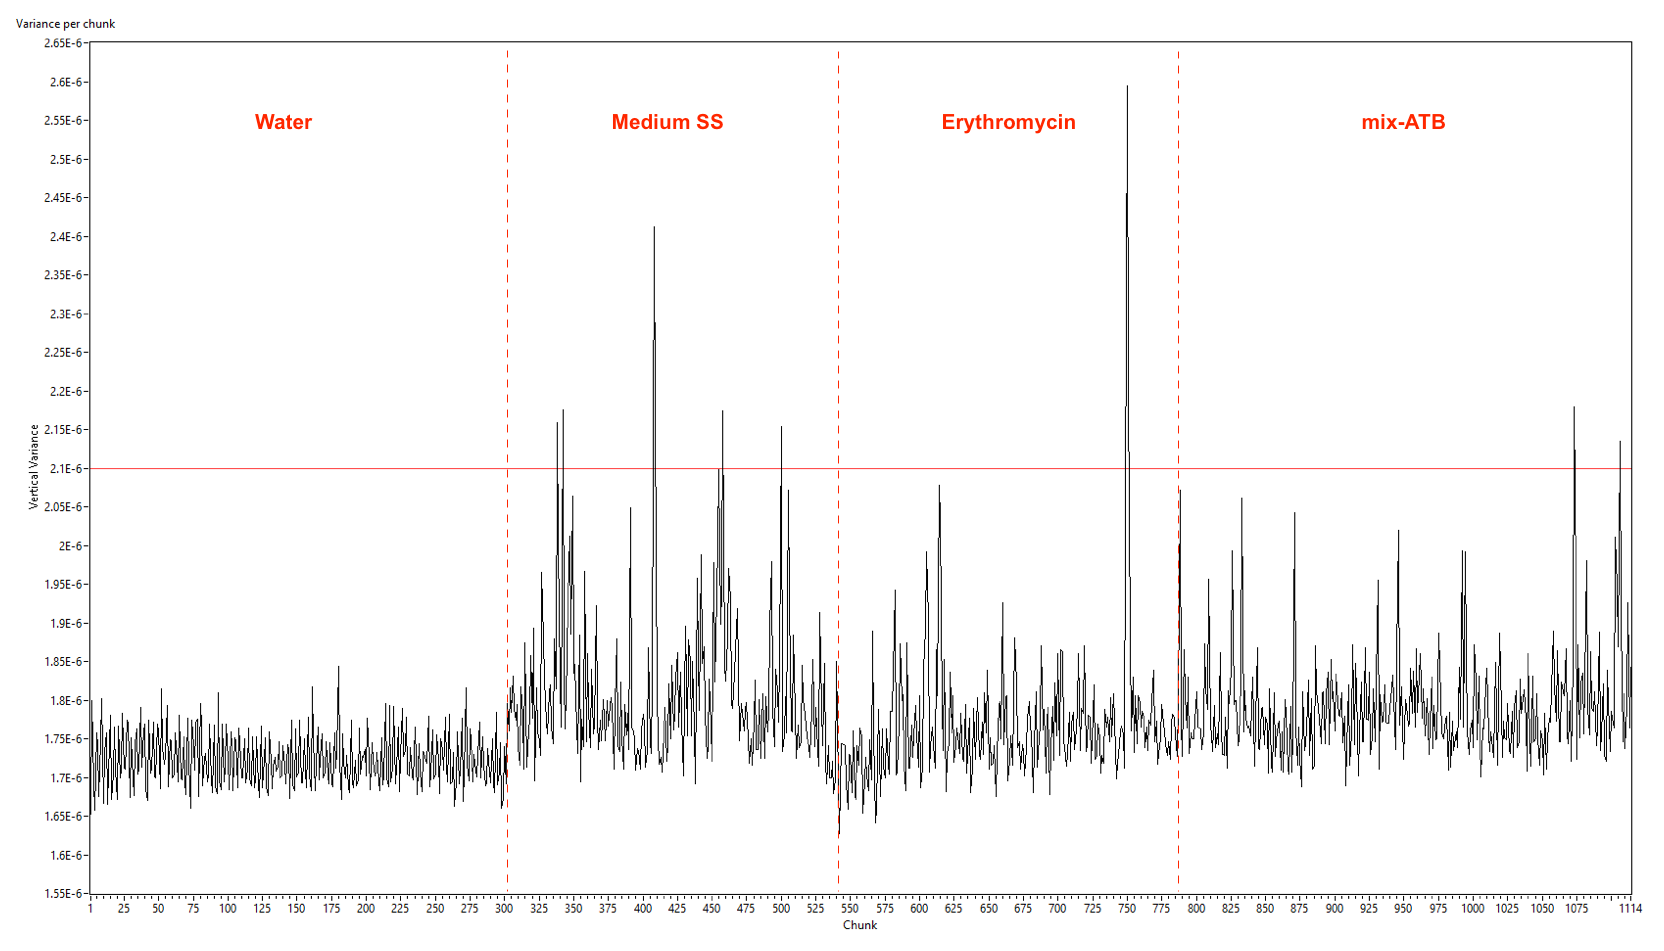
\includegraphics[width=1\linewidth]{Signal/Water_medium_atb.png}
\label{fig:water_med_atb}
\caption{Comparative activity of Water, SS medium, and two types of Antibiotics}
\end{figure}

We underline with that in general the activity of ATB are not affecting the activity of the cantilever compared to water. 
\begin{figure}[h]
\centering
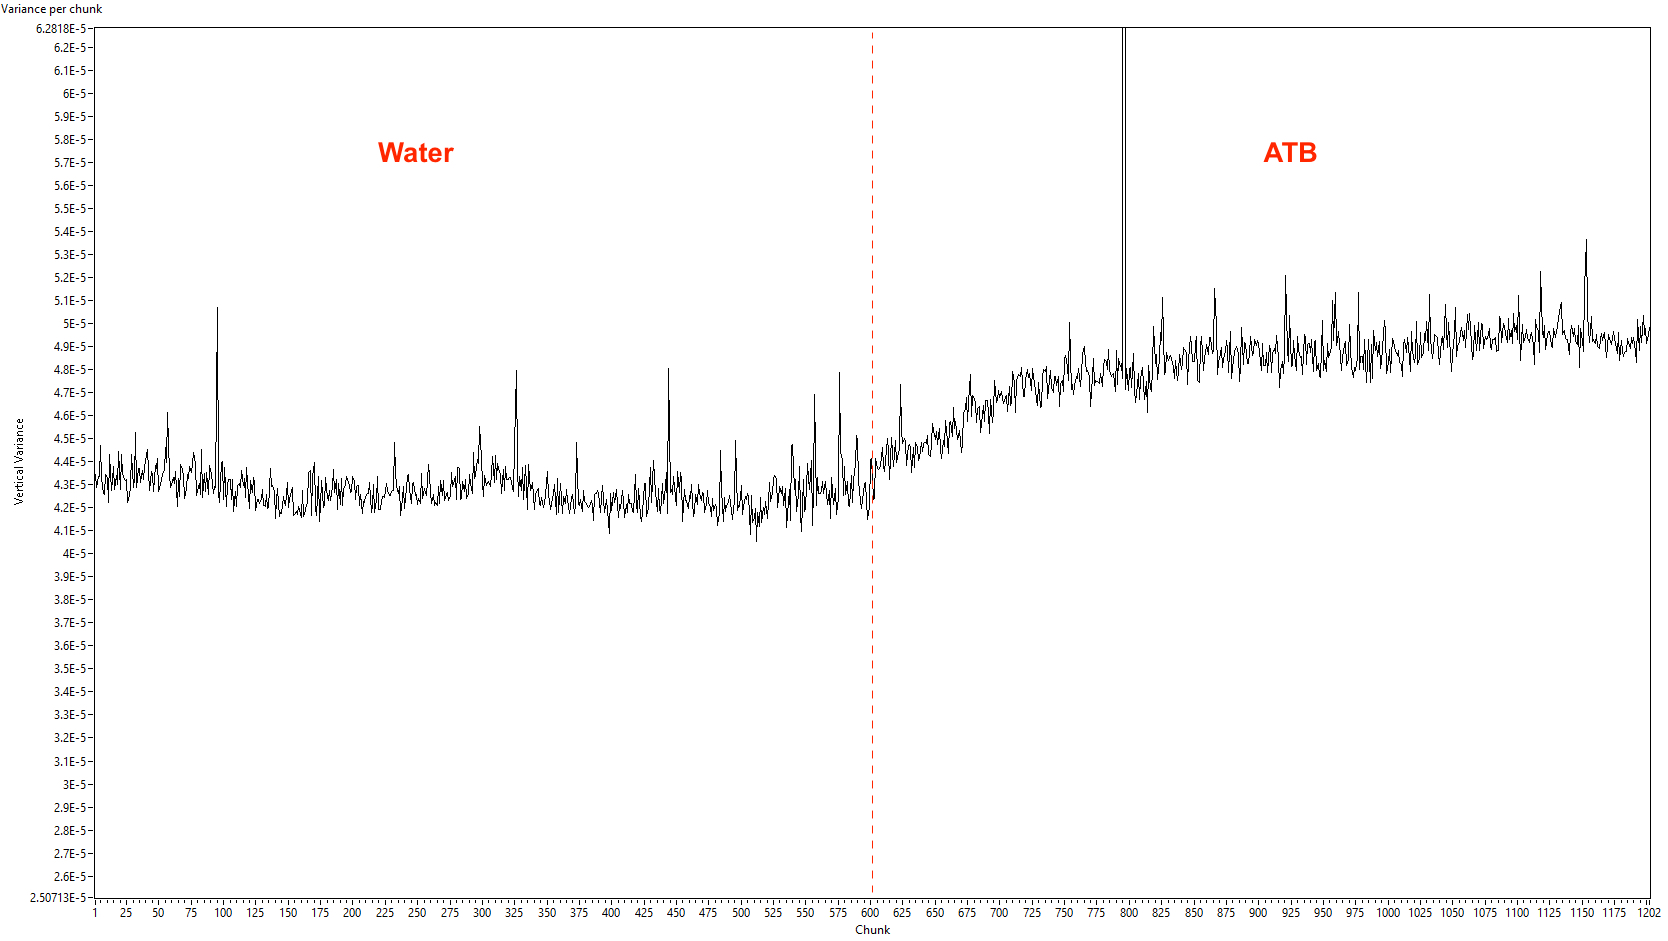
\includegraphics[width=1\linewidth]{Signal/Water__ATB2.jpg}
\label{fig:water_ATB}
\caption{Comparative activity of Water and Antibiotics}
\end{figure}
At least we tried to compare the activity of different concentration of medium (50\% and 100\%). 

%parte da riscrivere esperimenti non molto chiari...


% anche in questo caso potrebbe essere interesaante specificare nella discussione l'importanza della calibrazione per capire quanto é ampio il segnale rispetto ai batteri. 
  

\subsection{Bacteria and antibiotics}%-----------------------------------
	\subsubsection{E.coli}%----------------------
    The experiment has to be repeated...
    
	\subsubsection{B.Pertussis}%----------------------
The FFT of the first experiment\footnote{Experiment code: 280716} with Bordetella
show that the sensibility are always good (the pic on 4k Hz is always maintain) even if there is a small switch in the last part. 
\begin{figure}[h]
\centering
\includegraphics[width=0.7\linewidth]{FFT/FFT_280716}
\label{fig:FFT_280716}
\caption{FFT all along the experiment 280716, ATB1,2,3 are three different recorded time with the same ATB}
\end{figure}

For the first 20min after the injection of the ATB we can observe a normal activity of the bacteria (high variance). After this time the movement is still present but begin to decrease. We observe an optimal effect of the ATB ca. 1h after the injection and we need 2 hours to have a maximal effect of the Mix-ATB on BP. 
\begin{figure}[h]
\centering
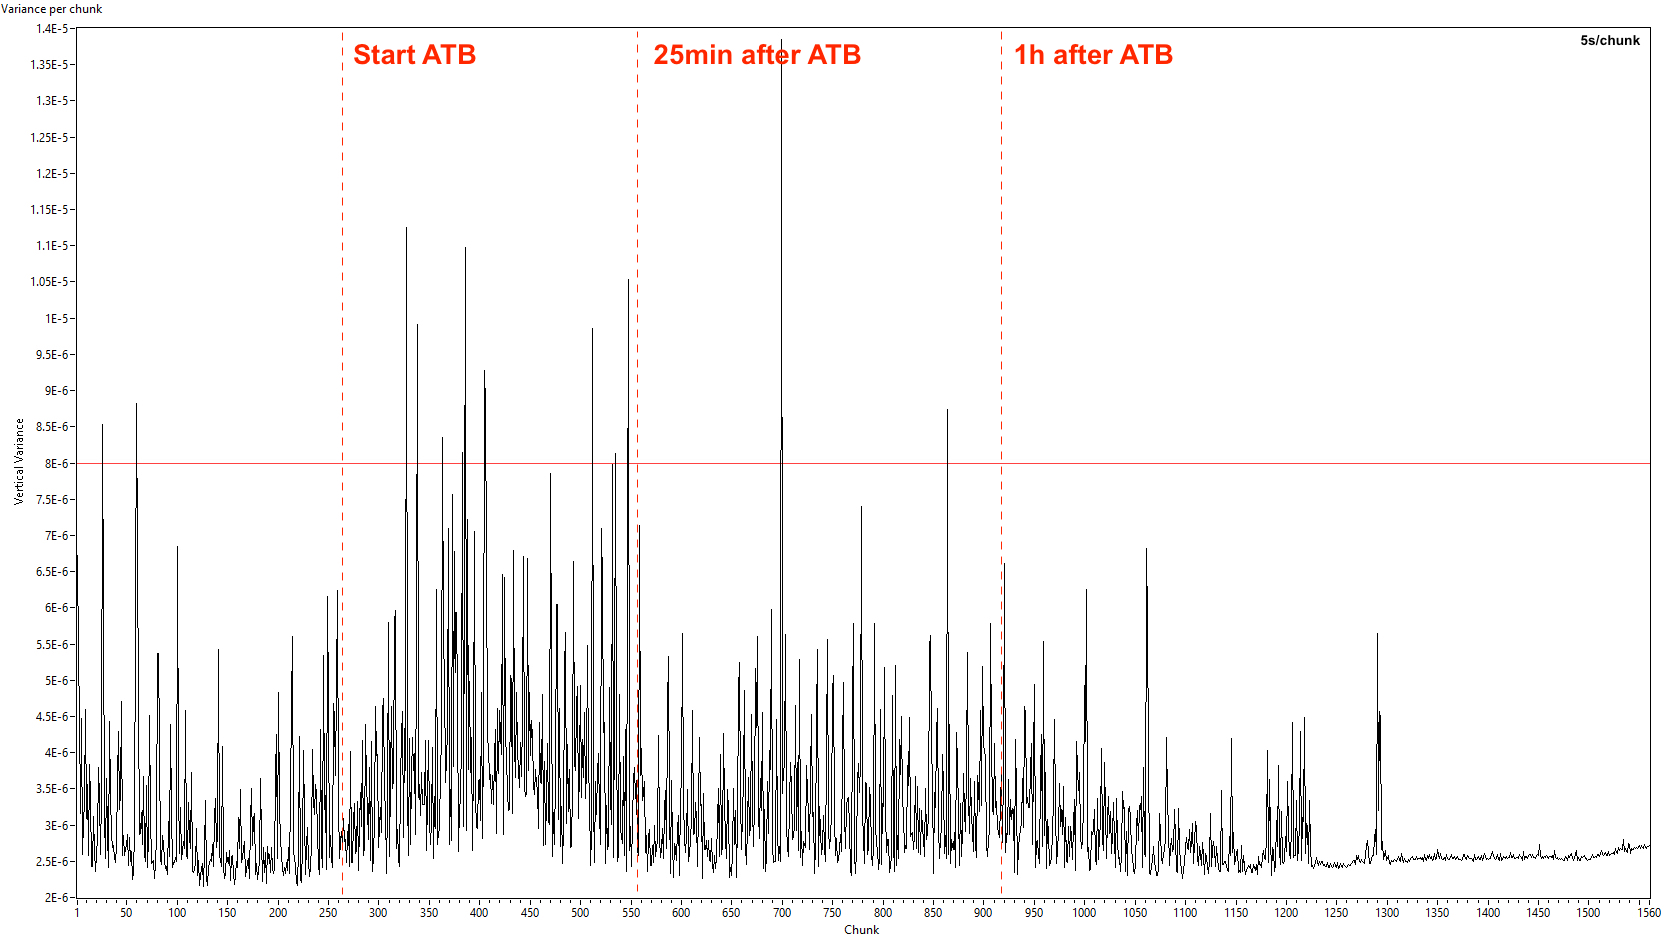
\includegraphics[width=1\linewidth]{Signal/sig280716.jpg}
\label{fig:Exp 280716}
\caption{Activity of BP and Mix-ATB}
\end{figure}
%controllare le tempistiche dello schema...

In the second  experiment\footnote{Experiment code: 020816} with BP  I had some problems with the FFT calibration in the first part, so it was difficult to estimate the movement  of the bacteria at the beginning. But I had a good FFT at the moment of the injection of the ATB. As the ATB need some time to have an effect on the bacteria we can consider the  movement at the time of the injection as the control movement. 
\begin{figure}
\centering
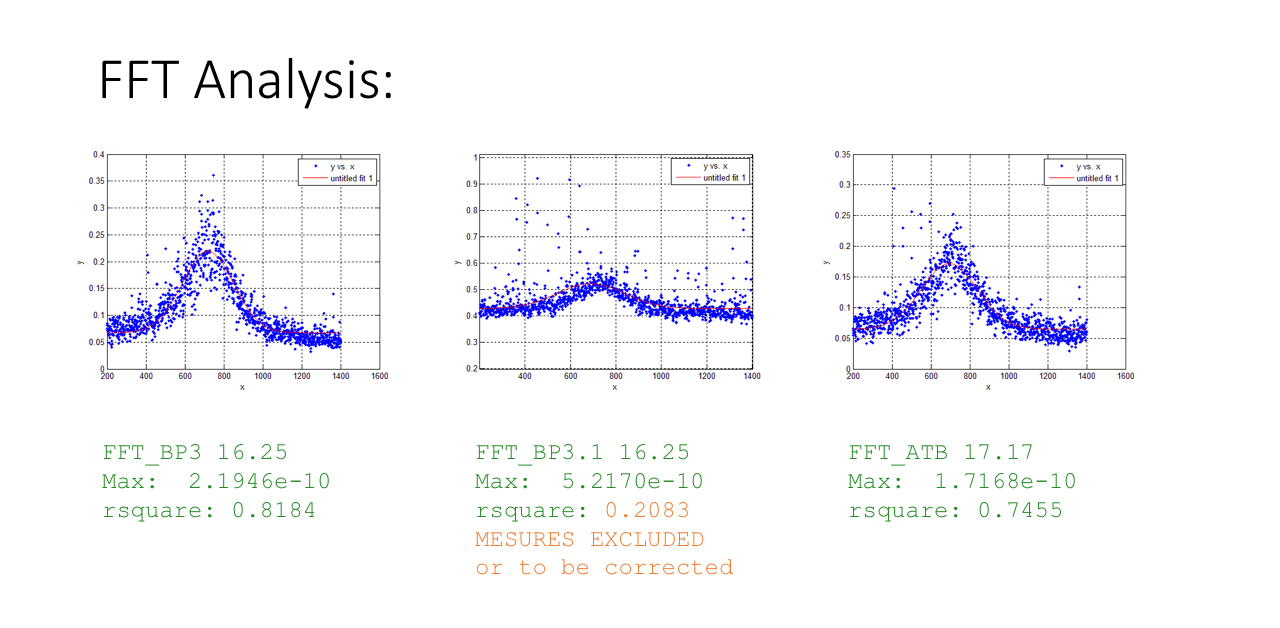
\includegraphics[width=0.7\linewidth]{FFT/FFT_020816.png}
%\caption{...}
\end{figure}
As in the first experiment we observe a decreasing of the activity about 30min after the injection but along the experiment (ca. 7h) we do not observe the maximal effect of the ATB. In this case the activity is decreased but maintain a minimal activity. 

We have observed the cantilever at the end of the experiment to understand what happened. 
\begin{figure}
\centering
	\begin{subfigure}{0.3\linewidth}
		\centering
		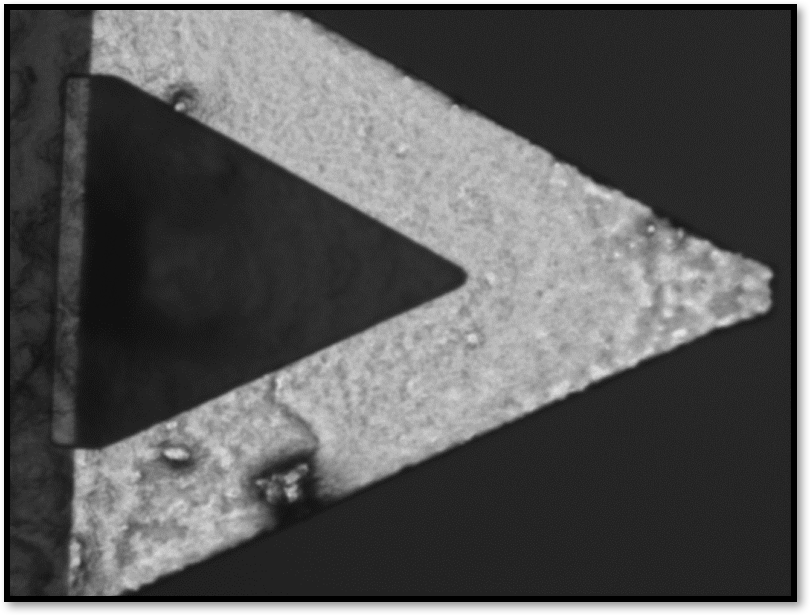
\includegraphics[width=1\linewidth]{Cantilever/Can020816_start.png}%[height=40mm]
		\caption{}\label{Can020816_start}
	\end{subfigure}
	\begin{subfigure}{0.3\linewidth}
		\centering
		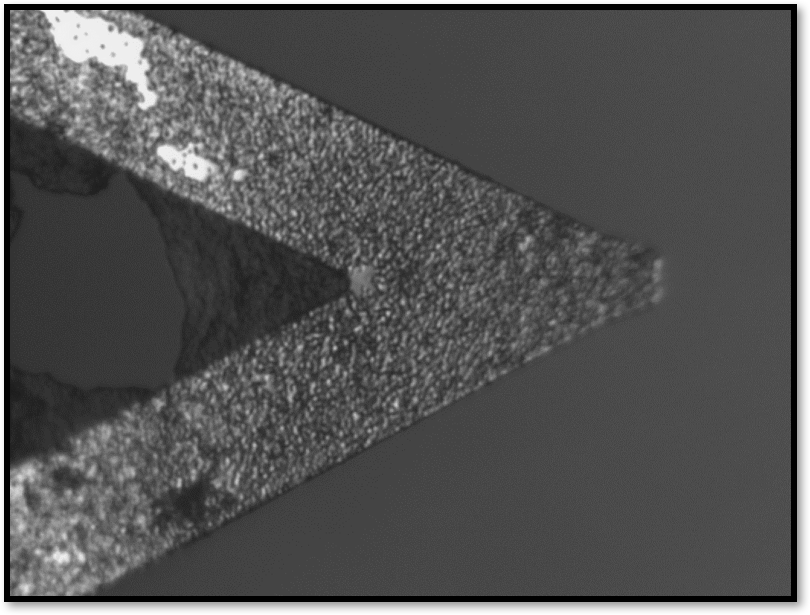
\includegraphics[width=1\linewidth]{Cantilever/Can020816_end.png} %[height=40mm]
		\caption{}\label{Can020816_end}
	\end{subfigure}
 \caption{Cantilever at the beginning \subref{Can020816_start} and at the end \subref{Can020816_end} of the experiment} 
  \end{figure}
%nelle conclusioni scrivere del dubbio di contaminazione


%\begin{figure}[]
%\centering
%\includegraphics[width=0.7\linewidth]{FFT_280716}
%\label{fig:Exp 280716}
%\caption{Activity of BP and Mix-ATB}
%\end{figure}

We usually observe a good effect of the MIC on BP\footnote{for example Experiment code: 160816}, always ca. in 1h. But in some experiments we observed that by injecting a second doses of ATB or using the MBC the activity temporally augmented and than decrease to a new basal activity. The new basal activity could be more important of the old one. 
%Discussion This could be correlated with the augmented liquid energy other with some molecular interactions with the cantilever.  
\begin{figure}[h]
\centering
%\includegraphics[width=0.7\linewidth]{...}
\label{}
\caption{Effect of MIC on BP}
\end{figure}

Also with the MBC alone we see a good effect of the ATB on the Bacteria in a relative short time. 
\begin{figure}[h]
\centering
%\includegraphics[width=0.7\linewidth]{...}
\label{}
\caption{Effect of MBC on BP}
\end{figure}

%The condition change when new solution enter the chamber or to many time pass. 
%The efficacy of the ATB is always good seen but is Difficult to isolate the effect of ATB and the different sensibility.

Finally in the experiment with the resistant strain of BP\footnote{Experiment code: 180816} we see that the movement in the medium and with the inefficient-ATB is always constant, even if the amplitude of the two sets are not comparable as with the inefficient-ATB (Erythromycin) the amplitude of the signal is more important as the one with medium (probably caused by the molecular interactions with the cantilever). But the important thing is that we observe the signal decreasing with the efficient-ATB (Mix-ATB at MBC concentration).
%importante commentare bene questo esperimento

\begin{figure}[h]
\centering
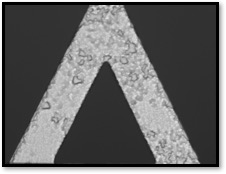
\includegraphics[width=0.3\linewidth]{Cantilever/Can180816.jpg}
\label{}
\caption{Resistant BP on cantilever}
\end{figure}

These experiments could be compared with the experiments of I. Vilalba 
	
    
    \subsubsection{Saccharomyces}%----------------------
    ...
    During the night we see an important increasing of the activity due to the grown of the yeast. In particular the presence of some little air bubbles could have increased the yeast metabolic activity\footnote{this suggest us that an other possibility to modify the metabolism of bacteria and yeast in addiction of giving nutriments could be to change the oxygen concentration of the solution for aerobic microbes}.
We see a great decreasing of the activity with the alcohol (the movement of the yeast is really important so the alcohol augmented reflection do not have the effect that has with bacteria) that the augmented reflection cover the bacterial minimal activity. This important decreasing has probably two components: 1° some yeast that has grown on the surface of the original one has detached during the changing of the medium. The second component is that the alcohol killed the yeast present on the cantilever that stopped the activity. 
with FFT (also with no correction) we know if the conditions are stable all along the experiment.  (Magari inserire un comment agli FFT di questo esperimento)

% inserire immagine segnale e FFT

\subsubsection{Free cantilever and bacteria suspension} %----------------------
   


\subsection{Algorithm for the normalization of the Signal}%---------------------------



%%%%%%%%%%%%%%%%%%%%%%%%%%%%%%%%%%%%%%%%%%%%%%%%%%%%%%%%%%%%%%%%%%%%%%%%%%%%%%
\section{Discussion}
We can imagine that we could make the calibration at each begin of experiment (after the alignment of the laser on the cantilever), or by turning on the prototype. A minimal vibration\footnote{or more small vibrations could be performed in different laser set point to have more points and calibrate more efficiently the function} will be performed when the laser is aligned in the optimal position (automatically) ant this point could be considered the optimal sensibility and the FFT will recorded (Optimal FFT). With this value we can set the \textit{c} value so that the function will be in the right position for this experiment (with the exponential part in the optimal position). With this calibration at the beginning of the experiment is possible to have a monitoring of the variation of sensibility of the prototype all’ along the experiment and in this way to correct the signal in a „theatrically standard sensibility “. An other interest of this calibration is that in this way comparison between experiments will be possible and more accurate. 
...
I found the same problem with hands-alcohol using S.Aureus but we had better rusults with pure alcohol. In particulary also with pure alcohol we have better results with SA and EC than BP. But the quality of the experiments are not enough representative as we can see with the comparison with Ines Vilalba experiments\footnote{annex} in witch the same results are not replicated. 

%%%%%%%%%%%%%%%%%%%%%%%%%%%%%%%%%%%%%%%%%%%%%%%%%%%%%%%%%%%%%%%%%%%%%%%%%%%%%%
\subsection{Bacteria and antibiotics} %------------------------------	

\subsubsection{E.Coli Experiments}
It could be interesting to quantify the quantity of metabolic energy of the bacteria from the amplitude of the signal (we need a normalization of the signal to compare the different value\footnote{see Calibration theory}) with a little theorem that consider the number of bacteria on the cantilever (counted with a program with an optic camera), their energy (after transformation from the vibration signal of the cantilever) and some other environmental parameters (like Temperature viscosity of the medium, reflaction ecc..)\cite{Danis idea}. 
The possibility of quantify the approximative metabolic energy of one bacteria could help us to detect one important caracteristic that could permit us to use a database to diagnostic the family of one bacteria starting from his movement (energy) pattern\cite{Sandor Idea of NeuronalMap}. \footnote{Questo probabilmente andrebbe nelle discussioni e non nei risultati}\\ In the same way we could modify the metabolism of aerobic bacteria with different fraction of oxygen in the medium and use the associated energy for each value of oxygen as an other parameter to identify the bacteria family\footnote{I do not investigate this ... but it could be a very interesting project for the future}.

\subsubsection{B.Pertussis}%----------------------
In the second experiment  I had difficulties with the  sensibility of the prototype in the first part. Analyzing the data I could understand that the problem in this part was the position of the laser on the cantilever. This problem was the point that  suggested me the idea of the calibration. 
%eventualmente inserire l'immagine con i laser e l'FFT
(...)\\
   We observe some difficulties be the change of the medium (change the position or density) that change the conditions and in this way also the sensibility (and the correspondent amplitude of the signal). For this reason is difficult to compare the amplitude of the different parts of the experiment but we can anly observe the trend of each experiment. We can see that with the medium and the first ATB we do not have a modification of the signal, instead with the mix-ATB we can observe that the signal is decreasing in intensity along the time. (SPIEGARE PIÙ CHIARAMENTE).

Definire delle soglie (% di attivita o intervalli di onfidenza) che ci dicano con una buona probabilità che il battere é morto e dunque l’ATB é efficace. 

\subsubsection{Saccharomyces}%----------------------
    (...)
As observed in the past, for long experiments is impossible to make a comparison of the amplitude of the signal between the beginning end the end because of the changing conditions (due to time and manipulations). For this reason without a calibration and normalization of the signal the only information we can (estrapolare) is the evolution of the activity in smaller peace of time (cambiare espressione).

\subsubsection{Free cantilever and bacteria suspension} %----------------------
    this is one of the most important series of experiment. As we could imagine that a clinical application cold be easier in this way. The isolated bacteria from the plasma (or infected spot-campione) is concentrated and entered in the chamber as we do in the experiment. It is easier that attach the bacteria on the cantilever and the quantity of bacteria are defined (or set) with the concentration\footnote{calculate with the…} and is more stable that the number of bacteria on the cantilever, that is really variable and difficult to monitoring. \\
Good detection of dead and alive bacteria movement but some liquids (like alcohol ) could make interference with the cantilever and cause a lot of movement (false +).
\\
\\
Problem with hand's alcohol:
\begin{itemize}
\item{Some molecules of alcohol or additional interfere with the cantilever causing movement.} 
\item{The density of the liquid ( normally don’t change because the alcohol was too diluted) change the laser refraction.}
\item{The molecules of alcohol or others molecules in the liquid went at the surface and deviate the laser (see image and schema) so the observed movement are not the one of the cantilever but more of the liquid surface\footnote{we can observe movement with a microscopic observation of the chamber with the camera}.}
\item{The alcohol is not a good way to kill bacteria as in high concentration (75\%) it destroyed the wall of the bacteria delivering a lot of small molecules and destroyed bacteria in the suspension that could cause important interactions with the cantilever. The same effect (important increasing of the activity) is observed with hand-alcohol disinfectant and pure 75\%alcohol.}
\end{itemize}

\subsection{Algorithm for the normalization of the Signal}%-----------------------------
%Potrebbe esser interessante inserire un calcolo della p-value/OR per vedere se c'é un cambiamento significativo prima/dopo la correzione o quant'é la differenza tra lo standard e il segnale corretto. O la differenza che c'é tra i risultati stessi. 

%Possibile mettere uno schema che descriva la sensibilità in rapporto alla posizioen del laser (vedi iphone) e agli altri parametri (ex viscosità).
Once we have found a good representative function we have to set it wit a calibration of the prototype at the beginning of the experiment. 
A possible calibration of the prototype could made having a small vibtation at the time with switch on the AFM (after having positionated the Cantilever and filled the chamber and the allignement of the laser with a good FFT pic) as an automatic set point. With this first vibration we could set the fonction in the right horizontal position by setting the \textit{c} variable: so that the starting FFT correspond to the hyperbolic part of the function (left extremites). We couldalso set the function with more little vibrations in sequences (for exmple 3 short vibrations for 3 variations of the laser position), that could ameliorate the precision of the function set point. \\The improvement of this system could permit us have a monitoring of the prototypoe sensibility (immagine con una linea di andamento della sensibilità in base al parametro utilizzato dell'FFT) and a correction of the signal that could make the results more consistent all the time long (it will be necessary to calculate a confidence intervall to know how good is the signal we have).\\
The differetn parameters of the function needed to be more deeply study to know how they react in each specific situation and change of (situazione ambientale) and more points are needed to have a more precise function. At the same time also the FFT have to be better studied to identify which parameter is better (indicante) the sensibility of the prototype. 

%QUESTI PASSAGGI DOVREBBERO ESSERE OTTIMIZZATI: TROVANDO UN ALGORITMO CHE INSERISCA L'AMPLIFICAZIONE SENZA AUMENTARE LA QUANTITA DI CALCOLO (da mettere nella discussione o conclusione)

% problema della calibrazione della scala x
% nei risultati specificare che il livello di fitting non é ancora ottimale e che potrebbe essere migliorato (migliore definizione dell'ampiezza della curva eccetera) e che lo scopo della funzione (migliorabile) é theorico, cioé per poter verificare se una correzione del segnale sia possibile. 
% generalizazione. Quindi la funzione verrebbe stabilita per ogni prototipo e punta e successivamente le due variabili rimarrebbero una modifica della verticale e dell'orizzontale (variabili C e D)
%Specificare che una delle cose pi?u importanti da fare sarebbe uno studio più approondito delk comprtamento degli FFT (per esempio la descrizione della miglior sensibilità e del rumore) e allo stesso modo uno studio più approfondito delle variabili della funzione come pure una migliore stima della funzione stessa (tutto questo nelle conclusioni). 
% la funzione deve essere quanto possibile "snella per permettere un calcolo di importantoi quantità di dati". 
%%%%%%%%%%%%%%%%%%%%%%%%%%%%%%%%%%%%%%%%%%%%%%%%%%%%%%%%%%%%%%%%%%%%%%%%%%%%%%
\section{Conclusion}
%%%%%%%%%%%%%%%%%%%%%%%%%%%%%%%%%%%%%%%%%%%%%%%%%%%%%%%%%%%%%%%%%%%%%%%%%%%%%%
The conclusion will be written at the end of the work...

%%%%%%%%%%%%%%%%%%%%%%%%%%%%%%%%%%%%%%%%%%%%%%%%%%%%%%%%%%%%%%%%%%%%%%%%%%%%%%
\section{Current State of the Work and upcoming works}
%%%%%%%%%%%%%%%%%%%%%%%%%%%%%%%%%%%%%%%%%%%%%%%%%%%%%%%%%%%%%%%%%%%%%%%%%%%%%%

per esempio: lavoro dennis sull'energia dei batteri
migliorare forula e algoritmo di calibrazione (studiare le variabili su più esperimenti)
Rifare studio sull'isolazione del rumore e della rumore elettronico sull'FFT
Studiare più a fondo il comportamento degli FFT 
Batteri: prvare con più branche resistenti . Determinare meglio l'effetto di MIC e MBC 
%%%%%%%%%%%%%%%%%%%%%%%%%%%%%%%%%%%%%%%%%%%%%%%%%%%%%%%%%%%%%%%%%%%%%%%%%%%%%%
\section{Abbreviations}
\begin{itemize}
\item ATB = Antibiotic
\item BP = Bordetella Pertussis
\item Mix-ATB = Trimethroprim and Sulfamethaxole (1:19)
\item SA = Staphylococcus Aureus
\item EC = Escherichia coli
\item SCM = Saccharomyces
\item SS = Medium of \textbf{Stainer and Scholte} for Bordetella Pertussis 
\item PBS = Medium of \textbf{Phosphate-buffered saline} for other Bacteria (E. Coli, S.Aureus, ...)
\end{itemize}
%%%%%%%%%%%%%%%%%%%%%%%%%%%%%%%%%%%%%%%%%%%%%%%%%%%%%%%%%%%%%%%%%%%%%%%%%%%%%%
\section{List of attachments}
\begin{itemize}
\item Code of Matlab script 
\item Images of strane cose
\item Isolazione del prototype
\item Pulitura della Punta 
\item Isolazione del rumore elettronico
\item List of experiment codes
\end{itemize}
%%%%%%%%%%%%%%%%%%%%%%%%%%%%%%%%%%%%%%%%%%%%%%%%%%%%%%%%%%%%%%%%%%%%%%%%%%%%%% MAGARI DA CANCELLARE
%\newpage
%\bibliographystyle{IEEEtranN}
%\begin{btSect}[IEEEtranN]{AnnualReport2014}
%\section{Scientific Publications, Presentations, Conferences}
%\btPrintAll
%\end{btSect}

%\begin{btSect}[IEEEtran]{BallisticVirtualSource}
%\section{References}
%\btPrintCited
%\btPrintAll
%\end{btSect}
\newpage
\begin{figure}%[b] = buttom
\centering
	\begin{subfigure}{0.245\linewidth}
		\centering
		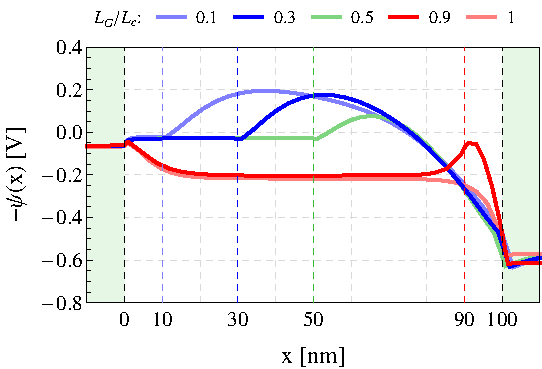
\includegraphics[width=1\linewidth]{potxPG100}
%		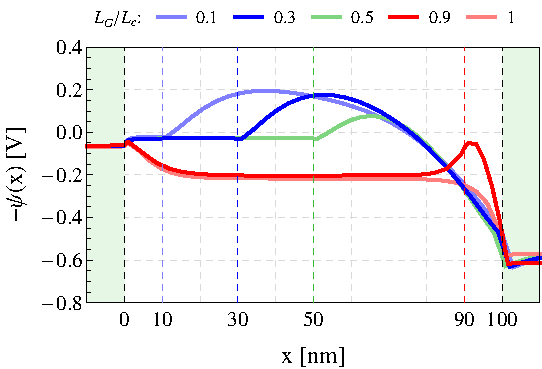
\includegraphics{potxPG100}
		\caption{}\label{fig:3:2a}
	\end{subfigure}
	\begin{subfigure}{0.245\linewidth}
		\centering
		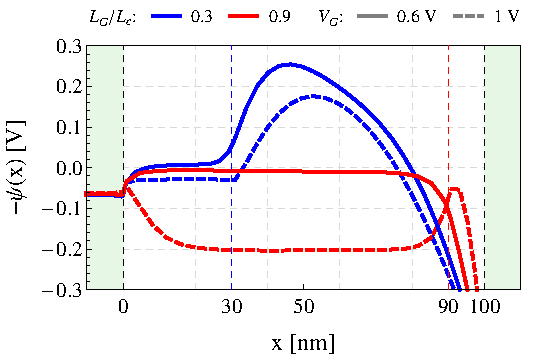
\includegraphics[width=1\linewidth]{potxPG100vg0610}
		\caption{}\label{fig:3:4a}
	\end{subfigure}
	\begin{subfigure}{0.245\linewidth}
		\centering
		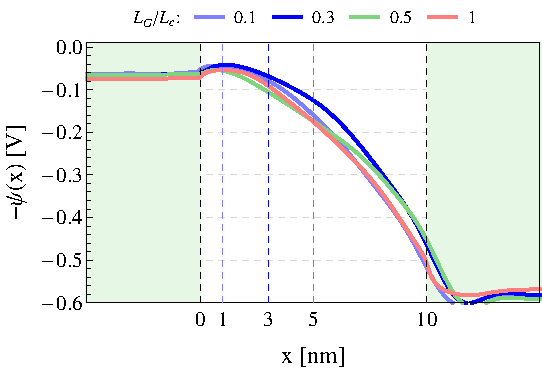
\includegraphics[width=1\linewidth]{potxPG10}
		\caption{}\label{fig:3:3a}
	\end{subfigure}
	\begin{subfigure}{0.245\linewidth}
		\centering
		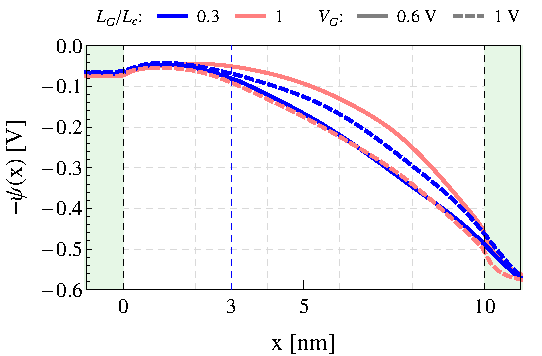
\includegraphics[width=1\linewidth]{potxPG10vg0610_new}
		\caption{}\label{fig:3:5a}
	\end{subfigure}
	\begin{subfigure}{0.245\linewidth}
		\centering
		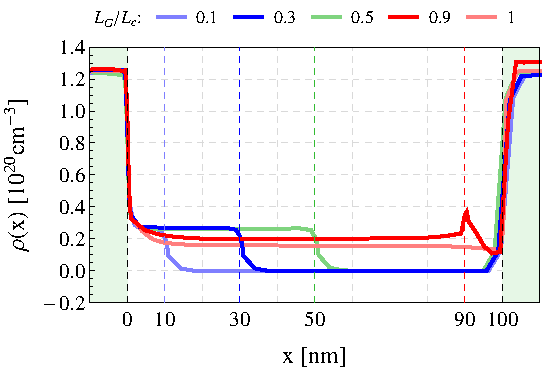
\includegraphics[width=1\linewidth]{ndxPG100}
%		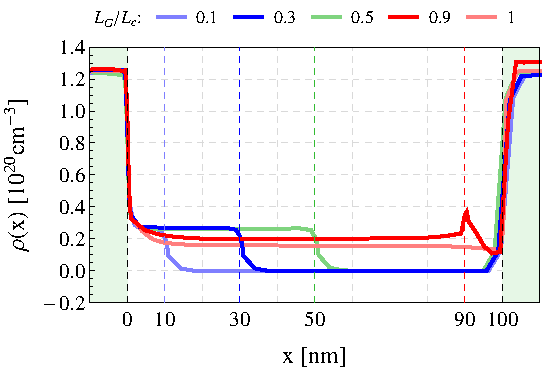
\includegraphics{ndxPG100}
		\caption{}\label{fig:3:2b}
	\end{subfigure}
	\begin{subfigure}{0.245\linewidth}
		\centering
		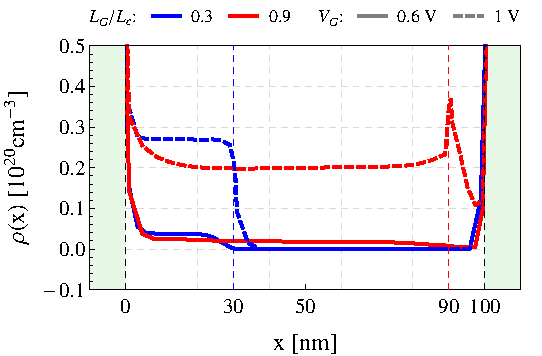
\includegraphics[width=1\linewidth]{ndxPG100vg0610}
		\caption{}\label{fig:3:4b}
	\end{subfigure}
	\begin{subfigure}{0.245\linewidth}
		\centering
		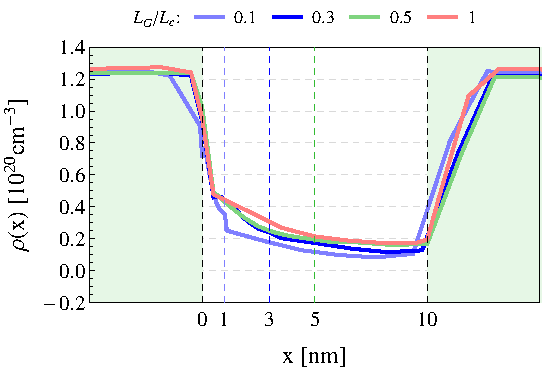
\includegraphics[width=1\linewidth]{ndxPG10}
		\caption{}\label{fig:3:3b}
	\end{subfigure}
	\begin{subfigure}{0.245\linewidth}
		\centering
		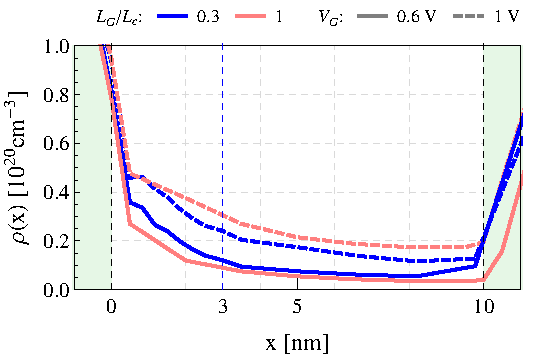
\includegraphics[width=1\linewidth]{ndxPG10vg0610_new}
		\caption{}\label{fig:3:5b}
	\end{subfigure}
	\caption{\subref{fig:3:2a},\subref{fig:3:4a},\subref{fig:3:3a},\subref{fig:3:5a} Potential
	profile \subref{fig:3:2b},\subref{fig:3:4b},\subref{fig:3:3b},\subref{fig:3:5b} Carrier density
	profile of the \SIlist{10;100}{\nm} partial-gate devices with different
	\nicefrac{L\sub{G}}{L\sub{c}} ratios.
	$\Vd=$\SI{0.5}{V}, $\Vs=$\SI{0}{V}}
	\label{fig:3:2}
\end{figure}%
%%%%%%%%%%%%%%%%%%%%%%%%%%%%%%% My Biblio %%%%%%%%%%%%%%%%%%%%%%%%%%%%%%%%%%
\newpage 
\begin{thebibliography}{9}

\section{Scientific Publications, Presentations, Conferences} %-----
\bibitem{Ban16} 
Ban Ki-Moon (UN General Secretary)
\textit{Global leaders commit to act on antimicrobial resistance}. 
\\NY City, 26.9.2016

\end{thebibliography}
%%%%%%%%%%%%%%%%%%%%%%%%%%%%%%%% Thanks %%%%%%%%%%%%%%%%%%%%%%%%%%%%%%%
\section{Thanks}
%%%%%%%%%%%%%%%%%%%%%%%%%%%%%%% Attachments %%%%%%%%%%%%%%%%%%%%%%%%%%%%%%%
\newpage
\section{Attachements}
\subsection{List of experiments} % bisogna mettere gli esperimenti in ordine

\begin{tabular}{|l|l|}
\hline 
\textbf{Code of Experiment:} & \textbf{Experiment description}\\ 
\hline
020816 & qui bisognerebbe commentare rapidamente ogni esperimento\\
\hline
060716 & ciao\\
\hline
070716 & ciao\\
\hline
080816& ciao\\
\hline
090816& ciao\\
\hline
110716& ciao\\
\hline
110816& ciao\\
\hline
120716& ciao\\
\hline
120816& ciao\\
\hline
130816& ciao\\
\hline
140716& ciao\\
\hline
150816& ciao\\
\hline
160816& ciao\\
\hline
170816& ciao\\
\hline
180816& ciao\\
\hline
250716& ciao\\
\hline
260716& ciao\\
\hline
270716& ciao\\
\hline
280716& ciao\\
\hline
290716& ciao\\
\hline
\end{tabular}

%------------------------------------------------
\subsection{Matlab scripts}
\subsubsection{FFT fitting}
function [gof,Max,Amplitude] = GausFit2(x, y, lcut, rcut)


%-----------------------------------------------
\subsection{Strane cose}%--------------------------------------------------
% da citare e da mettere in annesso come lavoro secondario
\subsection{Altro}%--------------------------------------------------------




%%%%%%%%%%%%%%%%%%%%%%%%%%%%%%%%%%%%%%%%%%%%%%%%%%%%%%%%%%%%%%%%%%%%%%%%%%%%
\end{document}


